\documentclass{optica-article}
\journal{opticajournal} % for journals or Optica Open
\articletype{Research Article}
\usepackage{lineno}
\usepackage{verbatim}
\usepackage{graphicx} %immagini ecc
\usepackage{float}
\usepackage{hyperref}
\usepackage{placeins}

\pagestyle{plain}
\begin{document}

\begin{center}
    \Huge \textbf{Technical Report}
\end{center}
\author{\centering NaoChallenge 2025}
\bigskip

\noindent
\textbf{For more information} \\

\noindent\textit{Visit our website} \href{https://www.naoartemis.altervista.org/html}{website}

\noindent\textit{See our} \href{https://github.com/NaoArtemis/ChallengeNao25}{repository}

\noindent\textit{Write an email to: }
\email{socialnaoartemis@gmail.com}

\bigskip

\begin{figure}
    \centering
    
\includegraphics[scale=0.10]{figures/logo_v3.png}
    \label{fig:logo_con_scritta}
\end{figure}

\tableofcontents

\vspace{10pt}

\newpage

\begin{abstract*} 
\vspace{5pt}
\noindent

The NaoArtemis project was developed for the NAO Challenge 2025 with the goal of promoting the advanced integration of technology into the sports sector, aiming to enhance the experience of both athletes and spectators. The mission of the project is based on the union between technological innovation and inclusiveness, with particular attention to accessibility and inclusion.

One of the main objectives is the optimization of athletic training through the use of the humanoid robot NAO. The robot will be able to monitor athletes’ movements, providing feedback to improve performance. In addition, biometric parameters such as heart rate and step count will be detected, with the aim of preventing injuries and supporting physical recovery processes. Athletes’ mental health will also be considered: NAO will take on the role of a virtual motivational assistant, offering positive reinforcement and personalized suggestions.

At the same time, the project aims to make the sports experience more inclusive for the audience, with a specific focus on people with disabilities. In particular, NAO will provide communication support for individuals on the autism spectrum by adopting Augmentative and Alternative Communication (AAC) systems, thus promoting interaction and active participation in sporting events.

Finally, in collaboration with the Audace sports club, the project foresees on-field experimentation of the proposed solutions, contributing concretely to the innovation of the sports landscape through the use of robotics and artificial intelligence.
\vspace{5pt}
\section{Methodology and Techniques Used}

\subsection{DevOps and Agile Methodology}
To manage the project and continuously monitor progress, the team adopted practices and tools in line with the principles of the DevOps (Development \& Operations) paradigm, which promotes integrated collaboration between software development and technological operations.

Development was organized according to the Agile methodology, which involves iterative and incremental planning. The main tasks were divided into sub-tasks, assigned to team members based on their specific skills and the goals of each project phase. This approach promoted greater operational efficiency, improving productivity and work organization.

The use of tools for planning activities, tracking progress, and organizing workflows ensured a clear distribution of responsibilities and effective communication within the team.  
At the same time, the project was managed and versioned through \textit{GitHub}, allowing the release of several improved versions over time.

\subsection{GitHub}
GitHub is a cloud-based platform that enables distributed management of source code, facilitating collaboration among developers within software projects. At the core of GitHub is Git, a distributed version control system that precisely records every change made to the code, enabling the parallel management of multiple versions of the project and preventing data loss.

Within the platform, projects are structured into repositories. Developers can perform cloning operations to obtain local copies of the repositories, make local changes, and synchronize them with the remote repository using commands such as \emph{commit} and \emph{push}.

Team collaboration is facilitated by advanced tools such as \emph{pull requests}, which allow proposing changes and submitting them for review before integration into the main branch, and by the \emph{issue tracking} system, useful for structured management of bugs, reports, and requests for new features.

To optimize work organization, the team adopted a modular repository structure, distinguishing two branches: one dedicated to code development (“coding”) and one for multimedia content (“social”).

\subsection{Attendance Management File}
To ensure effective management of project activities, the NaoArtemis team constantly monitored the presence and operational contribution of each member through a shared tabular system that summarizes aggregated data for each participant:
\begin{itemize}
  \item Total hours worked
  \item Number of actual attendance days
  \item Participation percentage relative to the total number of workdays 
\end{itemize}

This information was essential to evaluate individual commitment and to balance the workload, especially during the review of responsibilities. These are PCTO hours (Paths for Transversal Skills and Orientation), which are mandatory external training activities required for high school students.

Work organization followed an approach inspired by the startup/business model, with autonomous and efficient task management. This system made it possible to accurately quantify each member's contribution, providing an objective basis for analyzing the team's operations and for drafting the final documentation related to the NAO Challenge 2025.


\begin{figure}[H]
    \centering
    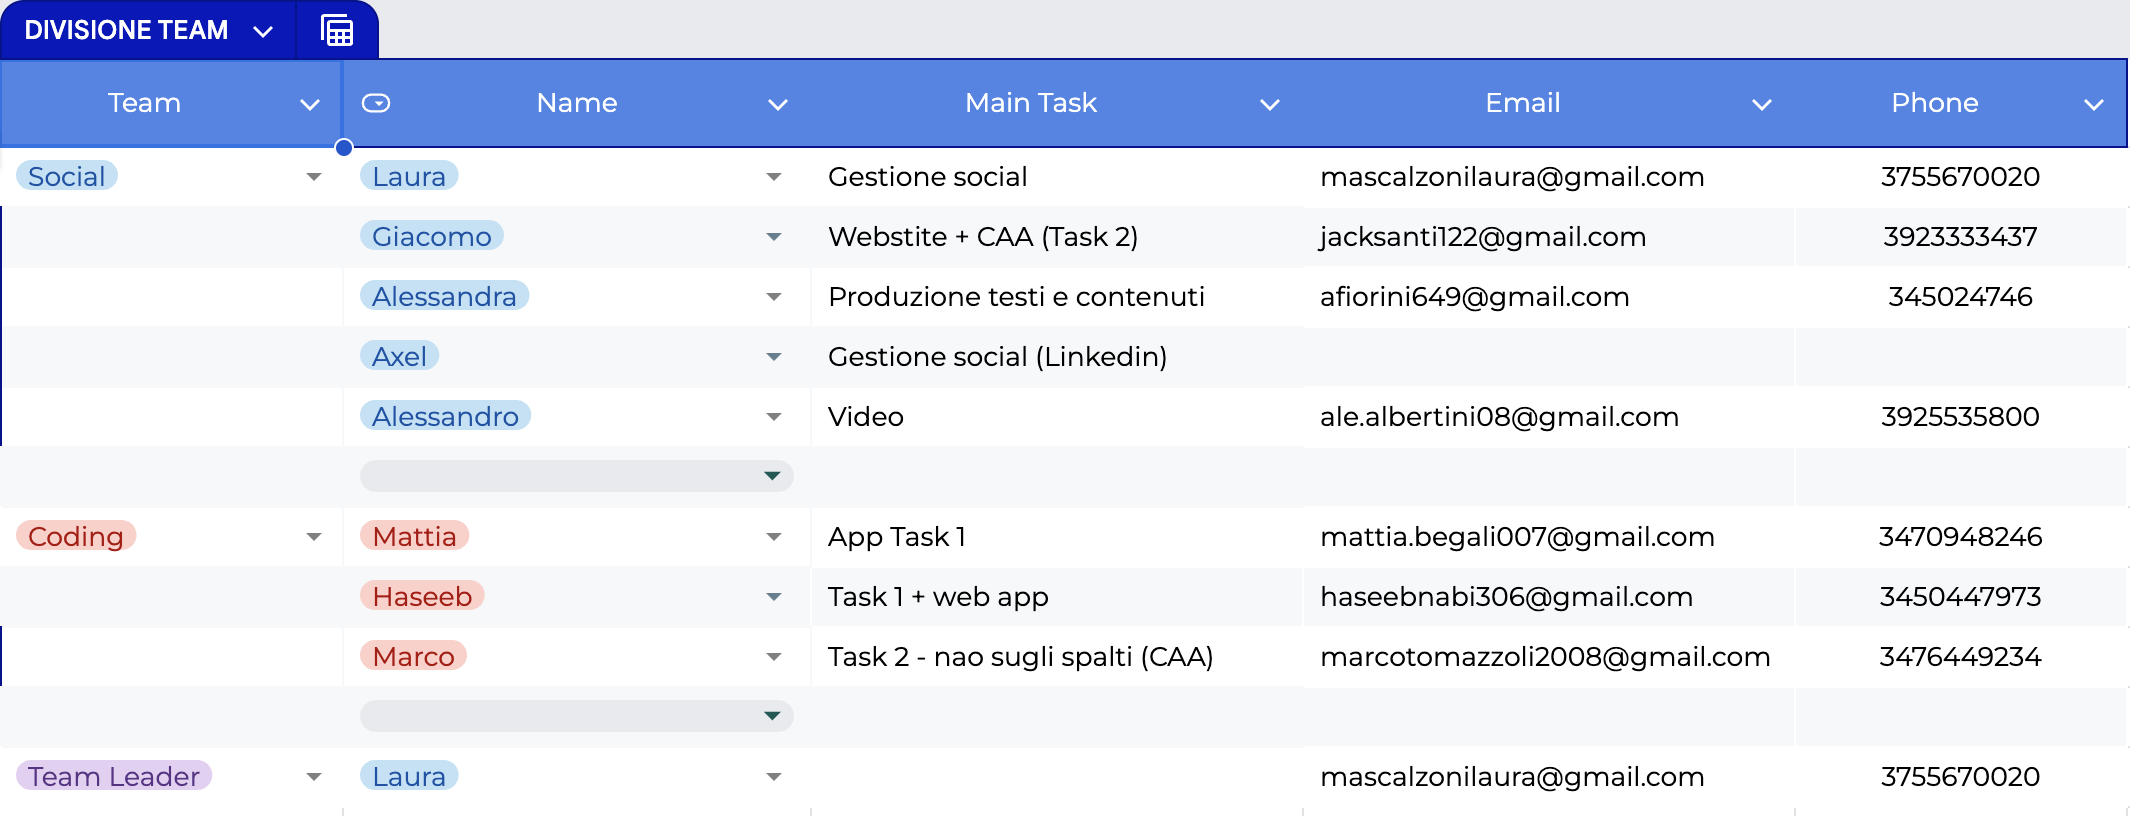
\includegraphics[width=0.9\textwidth]{figures/divisione_team.png}
    \caption{Table \texttt{TEAM DIVISION}: breakdown of members into respective teams, indicating main task, email, and phone number.}
    \label{fig:divisione_team}
\end{figure}

\begin{figure}[H]
    \centering
    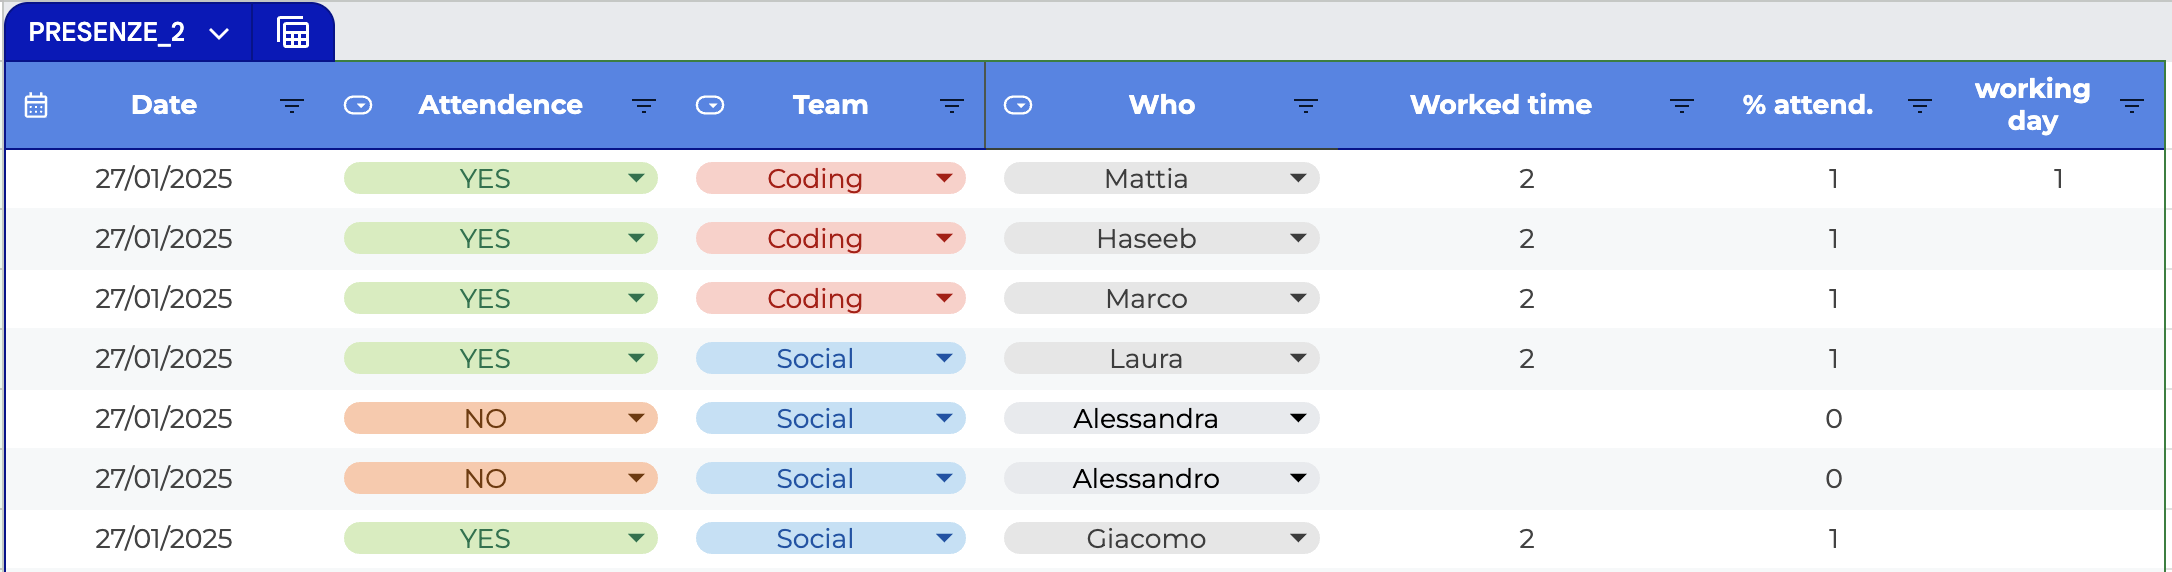
\includegraphics[width=0.9\textwidth]{figures/file_presenze.png}
    \caption{Table \texttt{ATTENDANCE}: daily attendance record of the team for the date 27/01/2025, indicating participation and team.}
    \label{fig:presenze}
\end{figure}

\bigskip

\noindent

\end{abstract*}

%%%%%%%%%%%%%%%%%%%%%%%%%%  body  %%%%%%%%%%%%%%%%%%%%%%%%%%

\section{Nao Challenge 2025 Project Description}

\subsection{From Challenge to Reality: NaoArtemis and the NAO Challenge 2025}
The NAO Challenge is an annual educational robotics competition aimed at high schools, technical institutes, universities, and research teams. The goal of the initiative is to promote the use of the NAO humanoid robot in the development of innovative technological solutions capable of addressing real societal needs. Through this challenge, participants are called upon to apply advanced skills in programming, artificial intelligence, interface design, and human-robot interaction in practical, multidisciplinary scenarios.

Each edition of the competition is centered around a specific theme designed to stimulate the design creativity and engineering approach of the teams. The 2025 edition focuses on sports: participants must design applications that use NAO's capabilities to optimize, personalize, or enhance the sports experience, both from the perspective of athletes and spectators.

The project focus includes aspects such as monitoring physical performance, supporting inclusion and accessibility, and using robotics to improve sports engagement and enjoyment. Participating in the NAO Challenge means facing a highly technological competitive context where it is essential to integrate technical skills with sensitivity to social and impactful issues.

\subsection{Meaning of the Name \text{NAO Coach \& Care (NC\&C)}}

The name \text{NAO Coach \& Care}, abbreviated as \text{NC\&C}, effectively and succinctly represents the dual purpose of our project for the NAO Challenge 2025.

On the one hand, the term \textit{Coach} highlights the role of the NAO robot as a technical assistant for the coach, capable of supporting tactical and physical analysis during matches and training sessions. On the other hand, the term \textit{Care} recalls the inclusive component of the project, which aims to improve accessibility in the stands for individuals on the autism spectrum, thanks to the robot's support and the use of Augmentative and Alternative Communication (AAC).

\subsection{Audace Supporting NaoArtemis 2025}
Audace Calcio a 5 Femminile, one of the most established and innovative sports organizations in the Verona area, is the official sponsor of the NaoArtemis project for the 2025 edition of the NAO Challenge. The club stands out nationally for its excellence in sports results and its multidimensional approach to athletic training, with a constant focus on the physical and mental well-being of its athletes.

The collaboration between Audace and the NaoArtemis team stems from a shared vision that places technological innovation in sports, inclusivity, and the promotion of youth talent at the center. In particular, Audace's support has enabled real-world testing of the project solutions, which integrate robotics and artificial intelligence to benefit performance, injury prevention, and accessibility in sports activities.

Thus, Audace confirms itself not only as a committed team on the field but also as an active partner in the development of new technologies serving women's sports, sustainability, and inclusion. Supporting the NaoArtemis project represents a further step toward a vision of sports as an evolutionary, educational, and socially responsible tool.

\begin{figure}[H]
    \centering
    
\includegraphics[width=0.6\textwidth]{figures/audace.png}
    \caption{Logo of Audace C5 Verona}
    \label{fig:audace_logo}
\end{figure}

\bigskip
\section{Task 1 -- Technical and Motivational Support for Athletes}

\subsection{Task 1 Description}
The first NAO robot will be configured to act as a virtual technical assistant, operating directly in the technical area. Its main functions include:

\begin{itemize}
    \item \text{Tracking and Analysis of Sports Movement}: using computer vision and motion tracking systems, the robot will be able to asynchronously analyze athletes' posture and motor dynamics, processing data collected during training and competitions at a later time.

    \item\text{Real-Time Biomechanical Analysis}:
    In the context of the project, biometric and biomechanical data are acquired using wearable devices (smartwatches), including heart rate (bpm), step count, and movement speed. The collected data are transmitted in real time and stored in a relational database based on \textit{PostgreSQL}, where they are structured in tabular format to enable queries, analysis, and further processing in a dedicated software environment.

    \item \text{Processing Tactical and Visual Data}: the collected data will be transformed into a single Voronoi diagram transmitted to the webapp, and used to generate personalized strategic suggestions for coaches, useful for studying opponents' matches or training sessions.
\end{itemize}

\subsection{General System Architecture}
The NaoArtemis system is structured according to a distributed architecture, composed of two independent servers developed in different Python environments to ensure full compatibility between the SDK components and advanced AI models.

\begin{itemize}
 \item The Python 2 server is exclusively intended for direct communication with the NAO robot, made possible through the use of the NAOqi SDK, which requires a Python 2.x environment for accessing the robot's low-level APIs. The official documentation available online was constantly consulted for development support: \url{http://doc.aldebaran.com/2-8/naoqi/index.html}.

  \item The Python 3 server hosts the Web Application and the infrastructure dedicated to the latest AI models. In this context, the following are active:
  \begin{itemize}
    \item YOLO for real-time detection and tracking of players and objects on the field;
    \item For each player, the average color of the uniform is calculated, and then the K-means algorithm assigns a team label (e.g., \text{red} or \text{blue}) based on color similarity;
    \item Voice generation of motivational messages or tactical communications via \text{OpenAI}'s \text{Text-to-Speech} APIs;
    \item An algorithm for tactical support aimed at suggesting real-time strategies during gameplay.
  \end{itemize}
\end{itemize}

The two servers communicate with each other via TCP/IP interfaces, ensuring synchronization between visual input, voice output, and athletes' status data. This configuration overcomes compatibility limitations between the NAO framework and modern AI tools.

\subsection{Computer Vision Techniques}
The "Assistant Coach" component integrates computer vision functionality, automatic tactical suggestions generation, and real-time monitoring of game parameters.

\begin{itemize}
  \item Sports scene analysis is performed using a system based on YOLO and K-means, which detect players and determine their position on the field via spatial coordinates (X, Y).
  
  \item Unlike a traditional heatmap, the system generates a single Voronoi diagram (Voronoi Soccer) representing each player’s area of influence on the field. This approach allows for more effective tactical visualization for the coach, highlighting coverage, free spaces, and positional imbalances.
  
  \item Biometric data received from the WebApp (heart rate, step count, average speed, etc.) are analyzed to assess the athlete's fitness level. The system can thus suggest real-time strategic substitutions, even in response to critical conditions (fatigue, performance drop, injury risk).
  
  \item Finally, an algorithm provides dynamic tactical suggestions, adapting gameplay based on opponent behavior and the field situation. The NAO robot can then transmit these indications to athletes through speech synthesis, making human-machine interaction more immediate and effective.
\end{itemize}

\subsection{Web Application}
The WebApp developed in the Python 3 environment is the management core of the system and allows control of the entire infrastructure through a responsive user interface, accessible via browser.

\subsubsection*{Main Features}
\begin{itemize}
  \item Injury management, with tracking of medical conditions and health history for each athlete;
  \item Match planning, event calendar, alerts, and pre/post-game statistics;
  \item Centralized database, which collects biometric, behavioral, and technical data, made accessible and updatable in real time by each module of the architecture.
\end{itemize}

\begin{figure}[H]
    \centering
    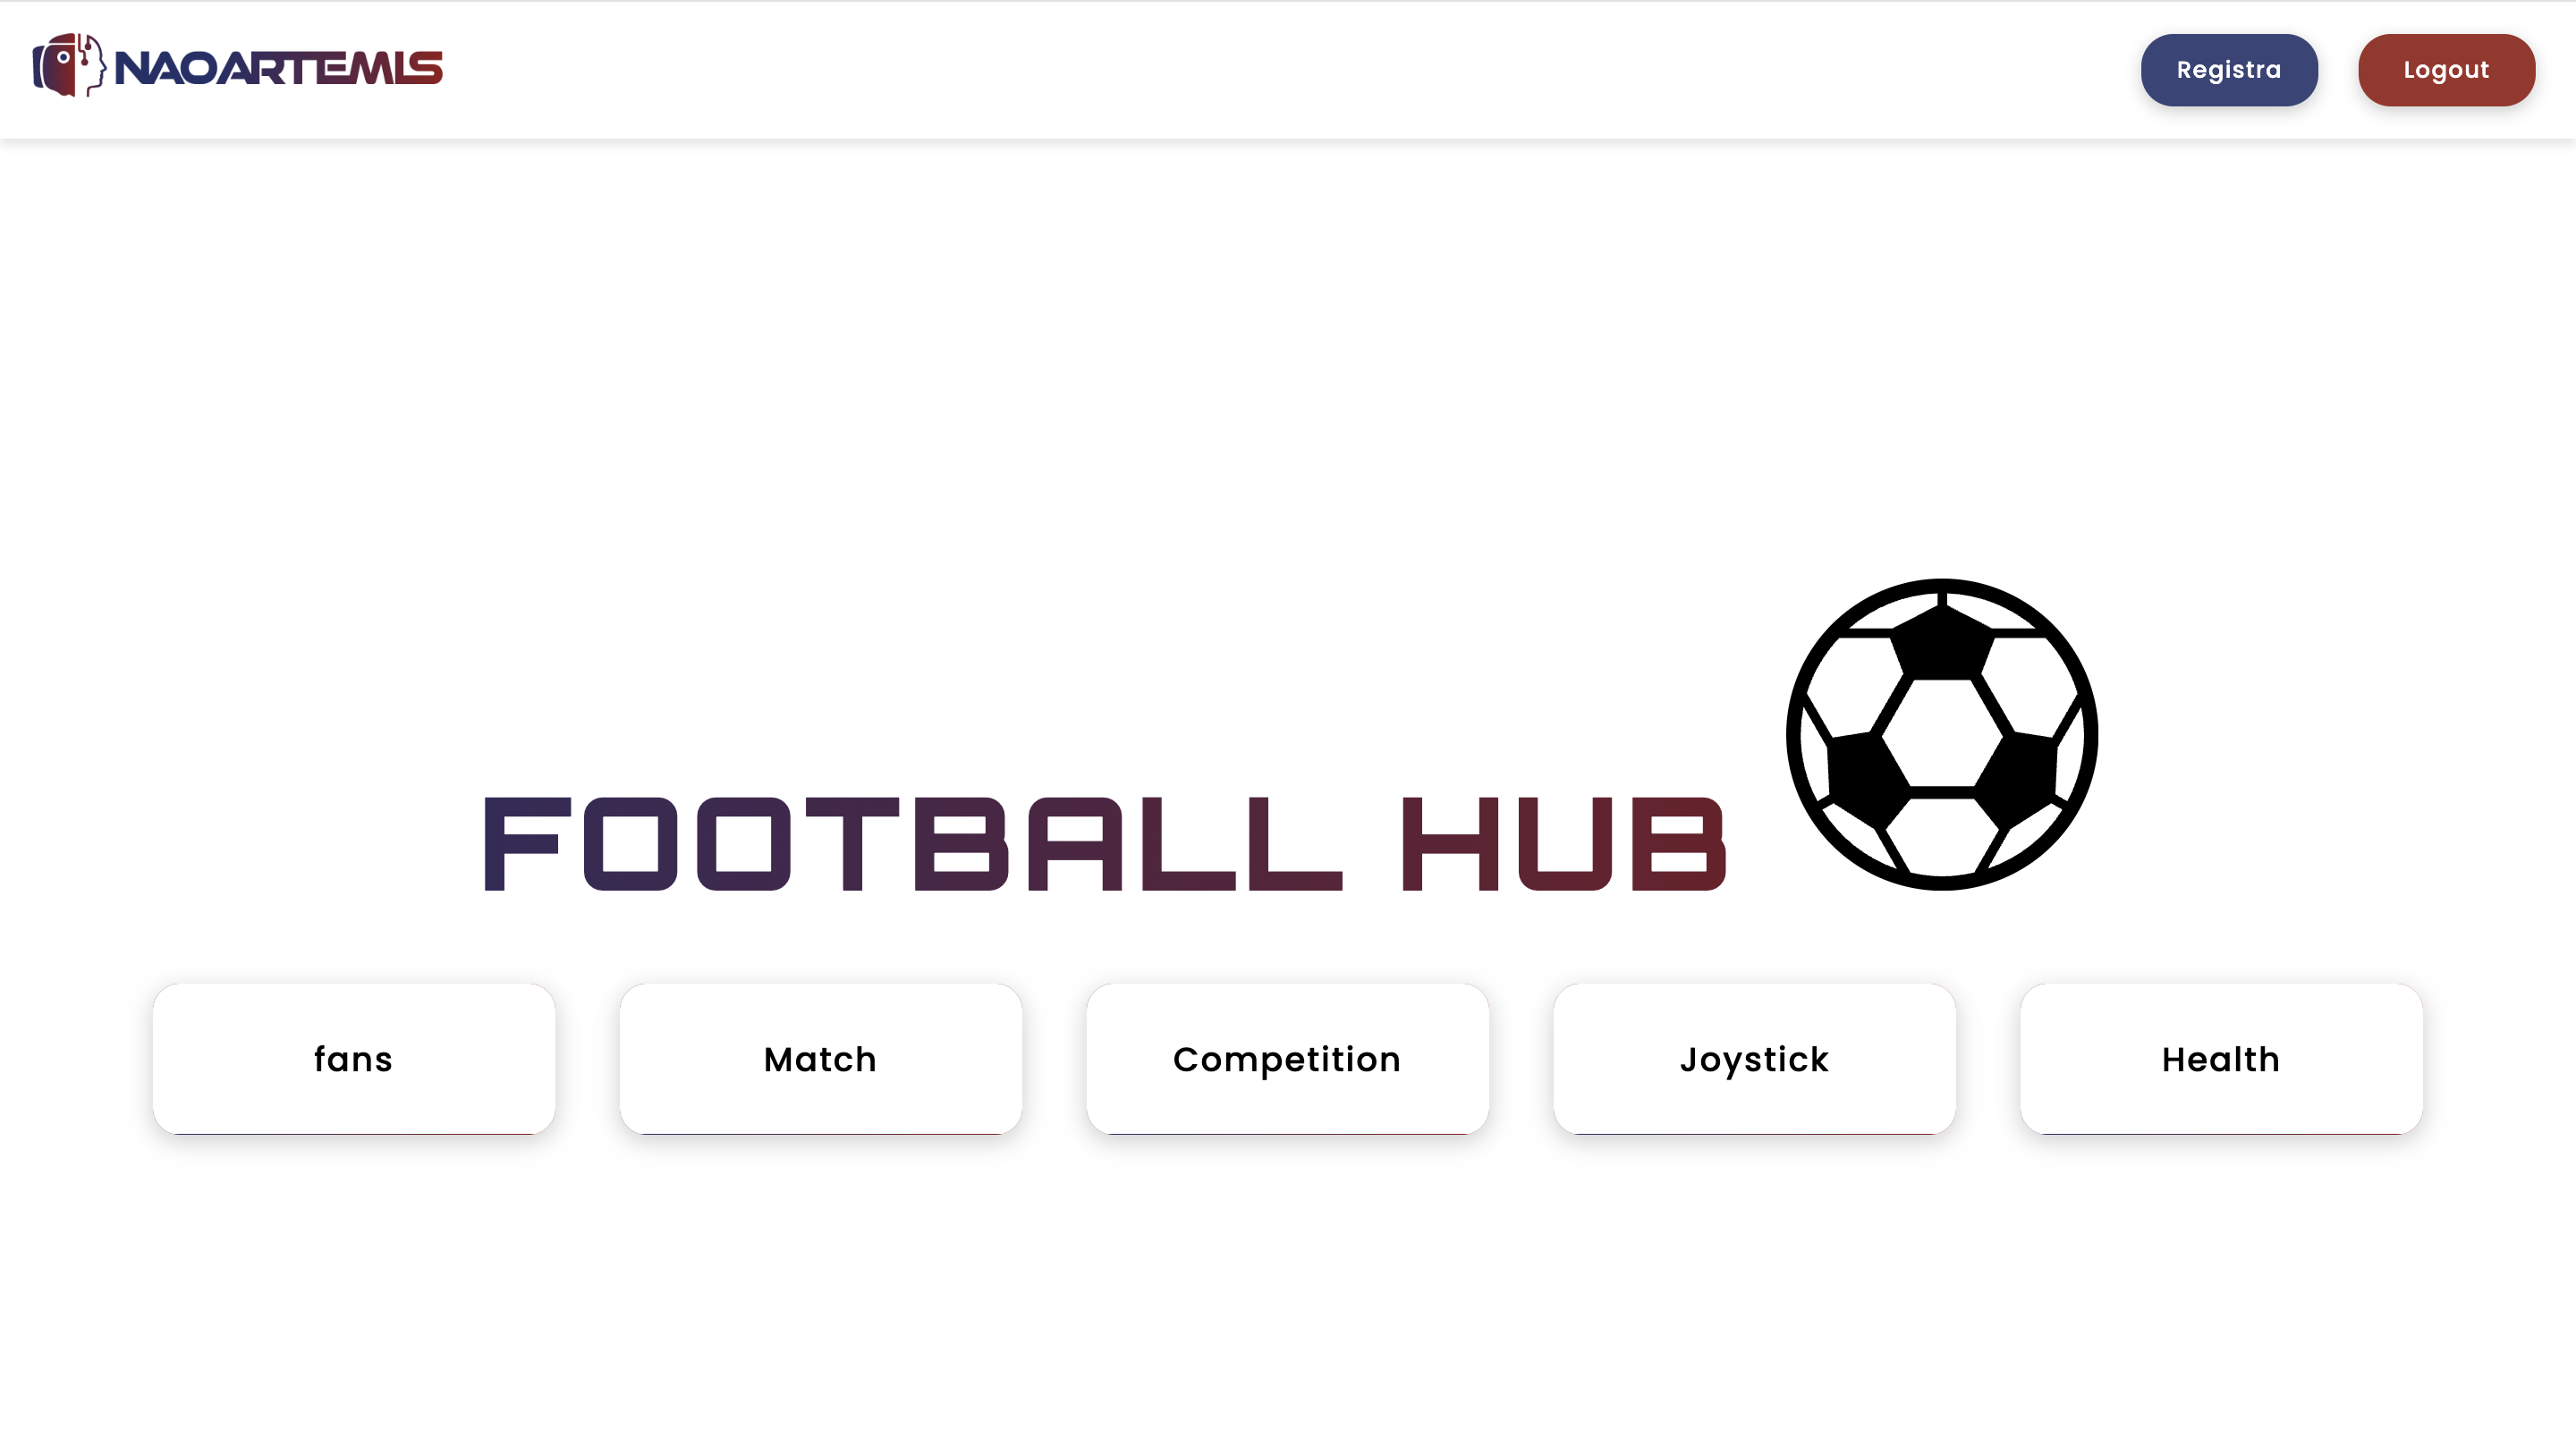
\includegraphics[width=\textwidth]{figures/homescreen.png}
    \caption{Home screen of the \textit{Football Hub} webapp, entry point to various functionalities: match management, competition, robot joystick control, and health monitoring.}
    \label{fig:home-screen}
\end{figure}

\begin{figure}[H]
    \centering
    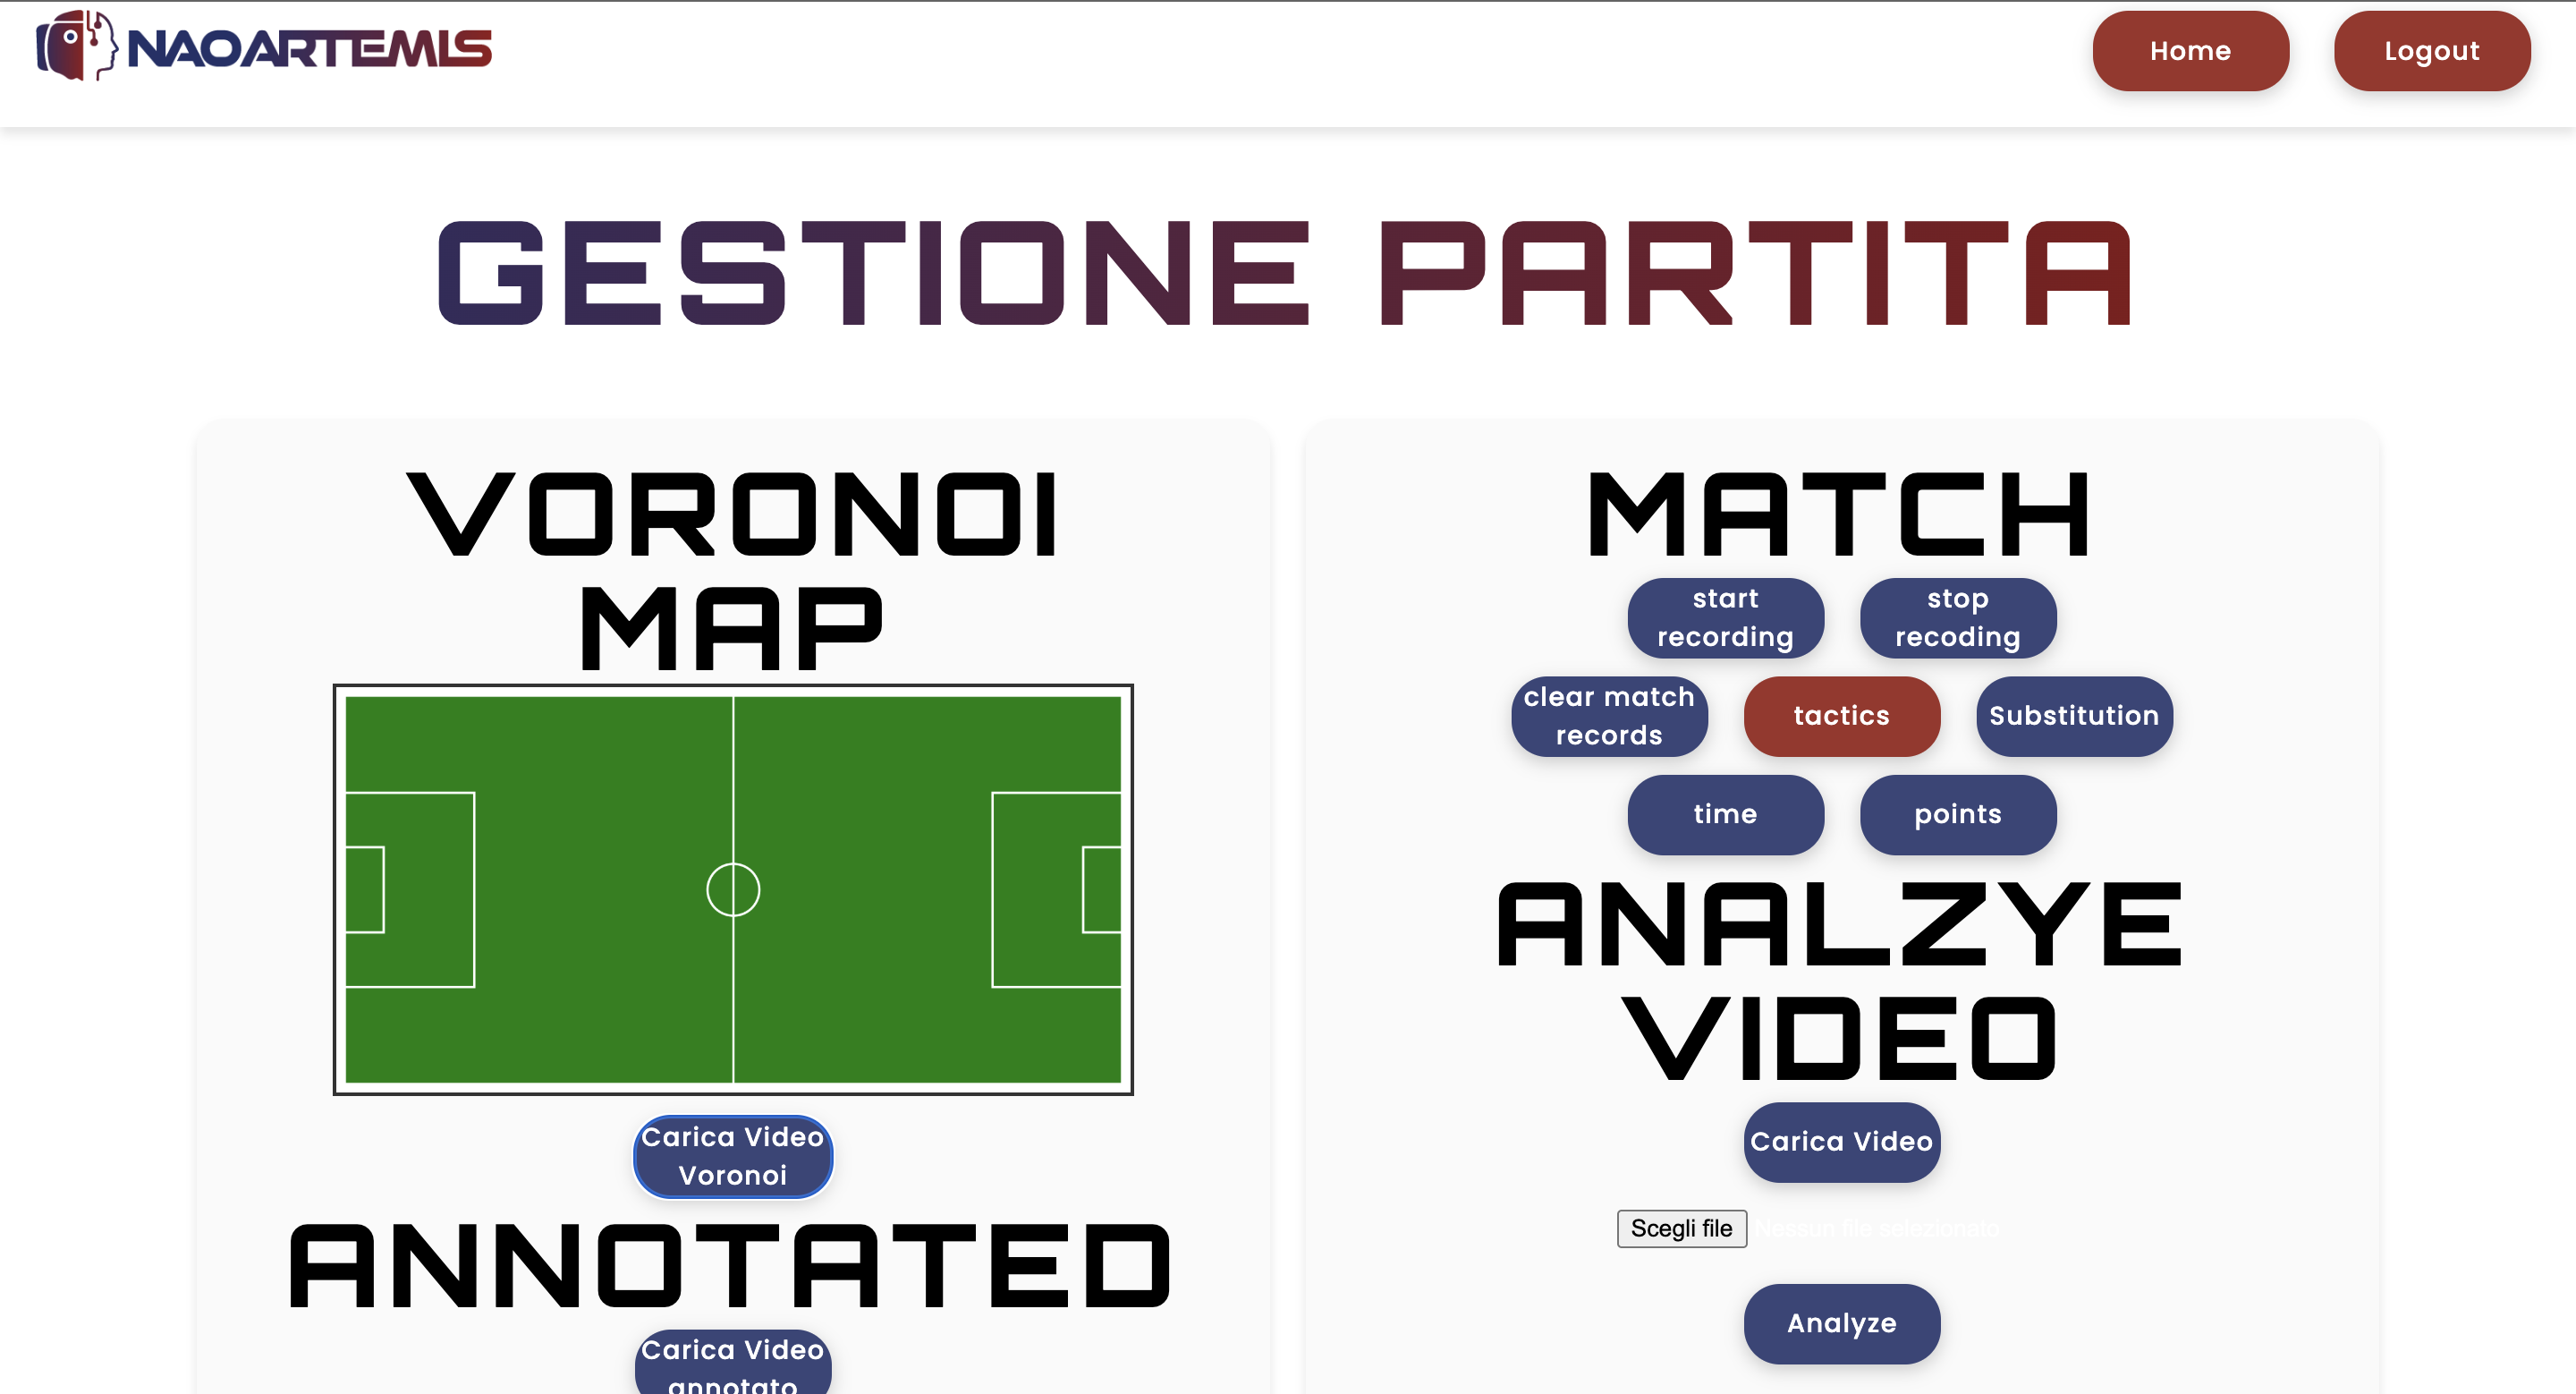
\includegraphics[width=\textwidth]{figures/gestione_partita.PNG}
    \caption{“Match Management” section of the webapp, which allows video uploads for tactical analysis.}
    \label{fig:gestione-partita}
\end{figure}

\begin{figure}[H]
  \centering
  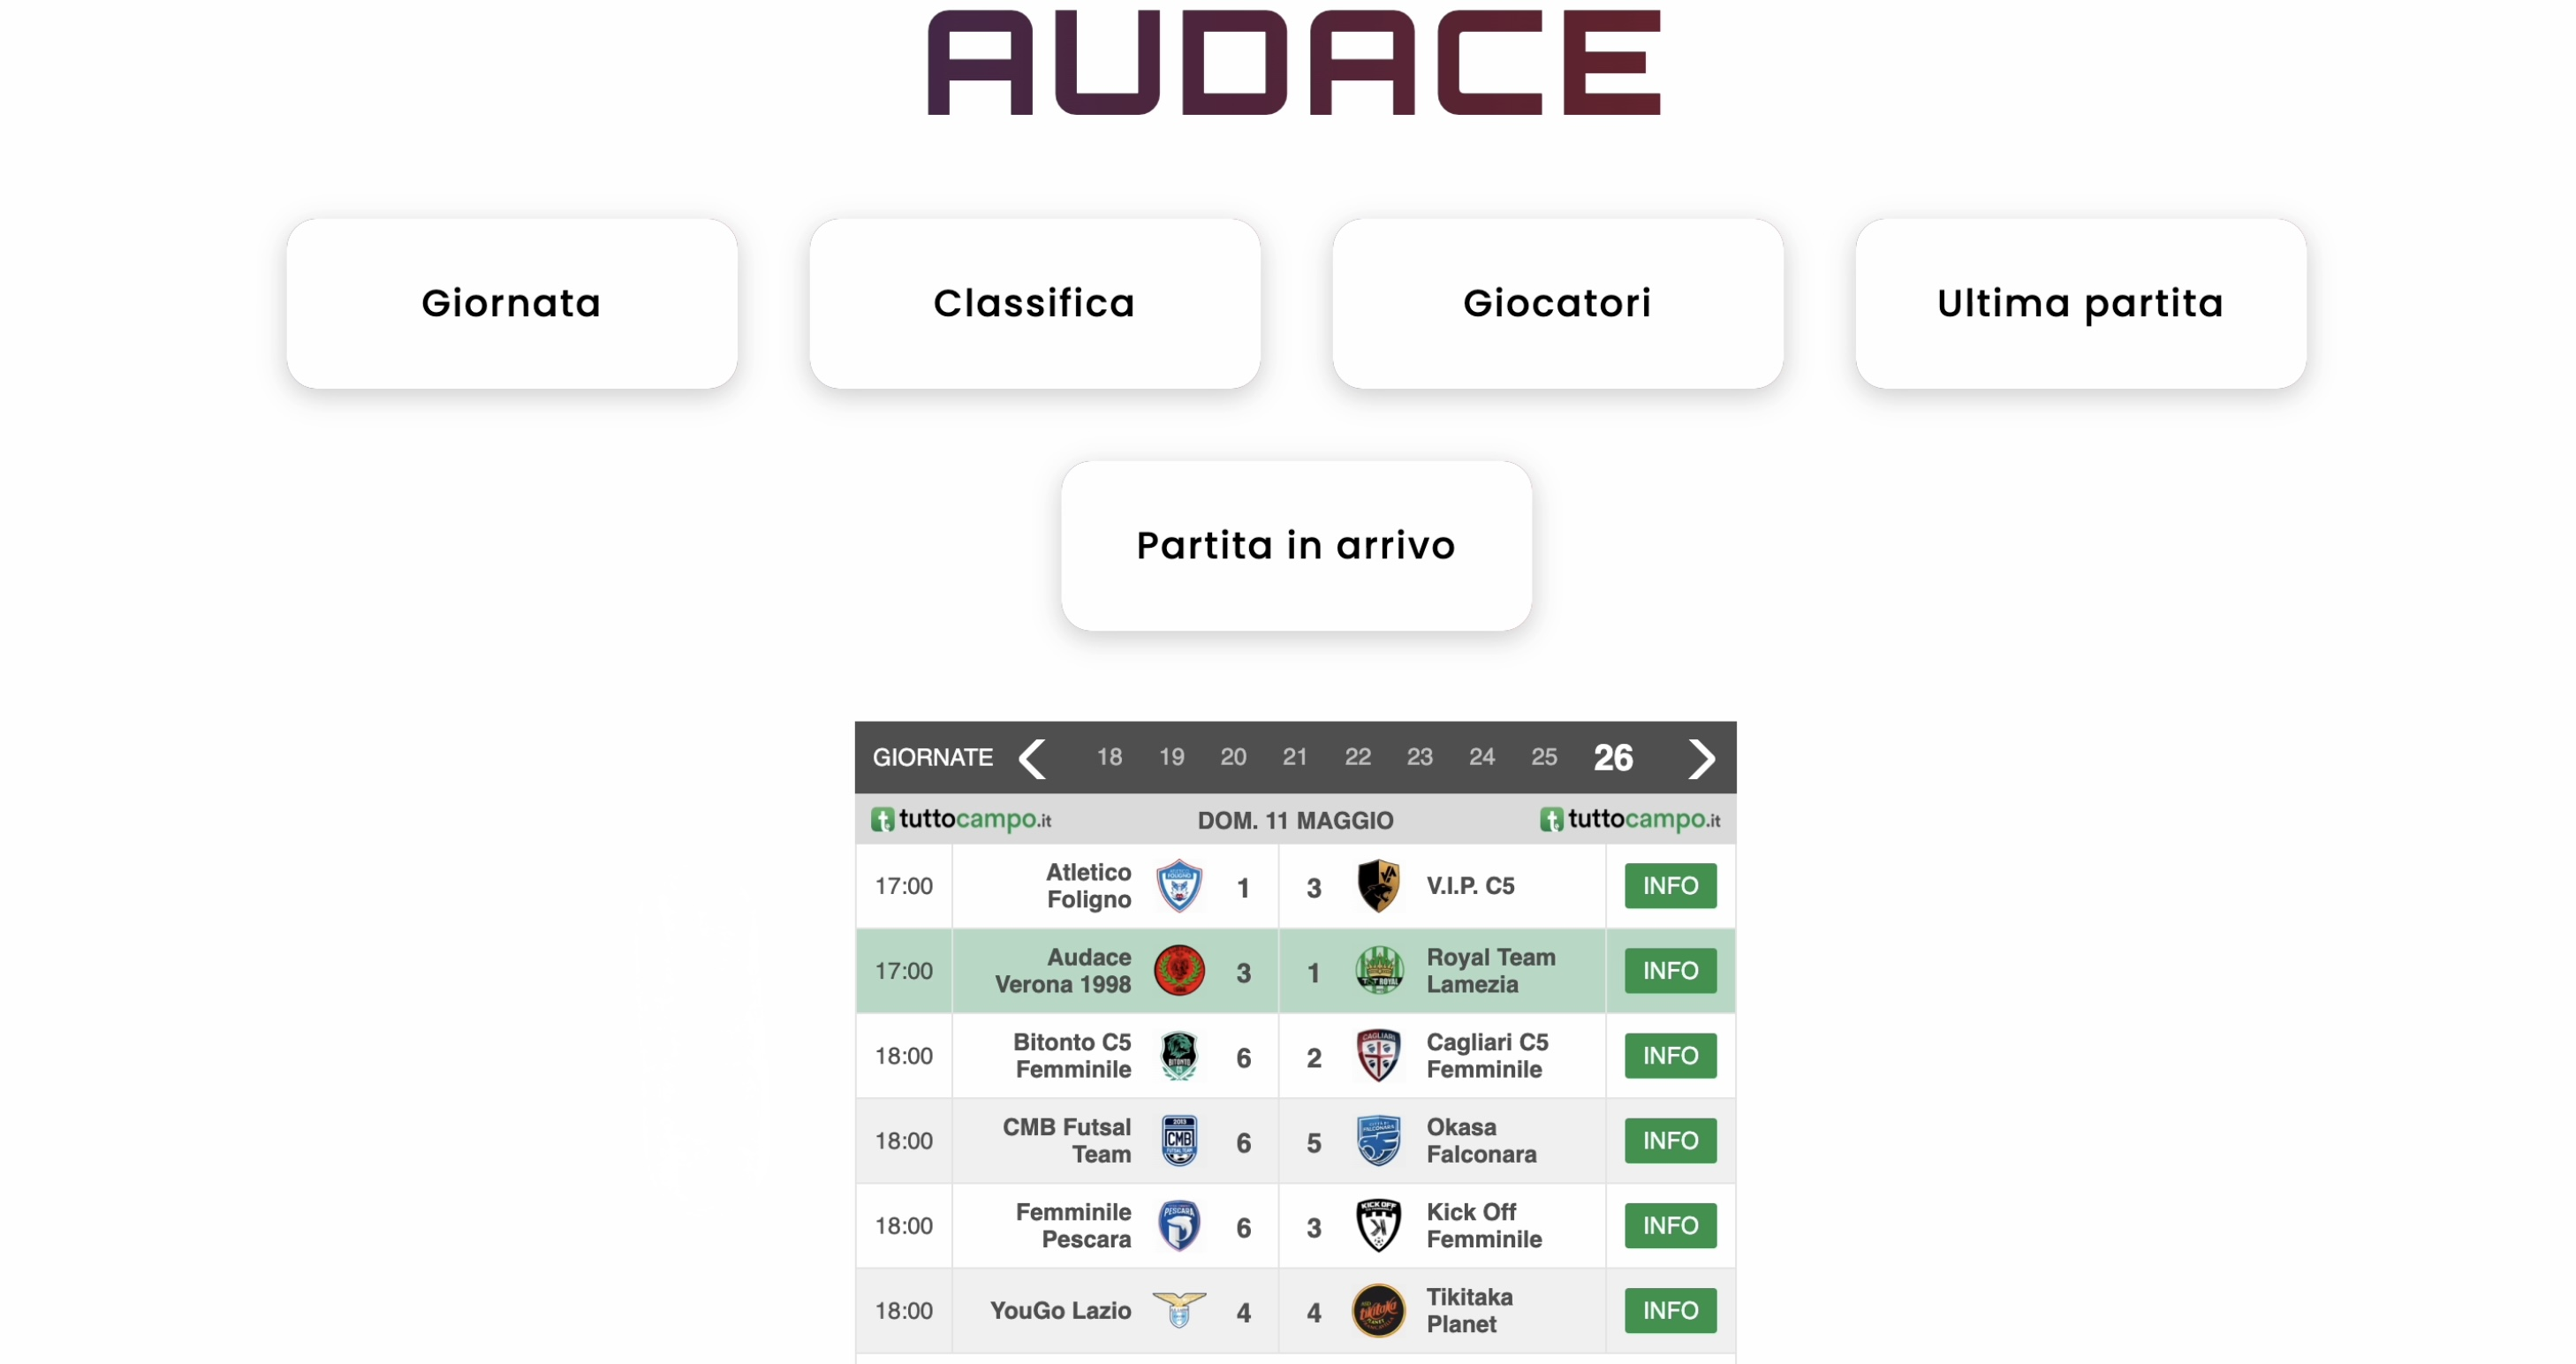
\includegraphics[width=\textwidth]{figures/audace.jpg}
  \caption{Section dedicated to the matchday and results of Audace’s match.}
\end{figure}

\subsubsection*{Manual control}
To offer maximum control and flexibility to the user, the team decided not to adopt Choregraphe, the official software for programming the NAO robot, due to certain technical and operational limitations. Instead, a system of essential but strategic manual commands was developed through the WebApp. This module allows the user to:

\begin{itemize}
  \item Enable/disable video streaming;
  \item Start ArUco recognition;
  \item Send voice messages;
  \item Directly and flexibly control NAO's basic actions.
\end{itemize}

\subsubsection*{Technical appendix: video processing components}

\paragraph{Python 3 Pipeline}
Processing of the recorded video stream using OpenCV and decoding of JPEG frames. The frames are analyzed *after* the match using computer vision models (such as YOLO and KMeans clustering).

\FloatBarrier

\begin{figure} [H]
\centering
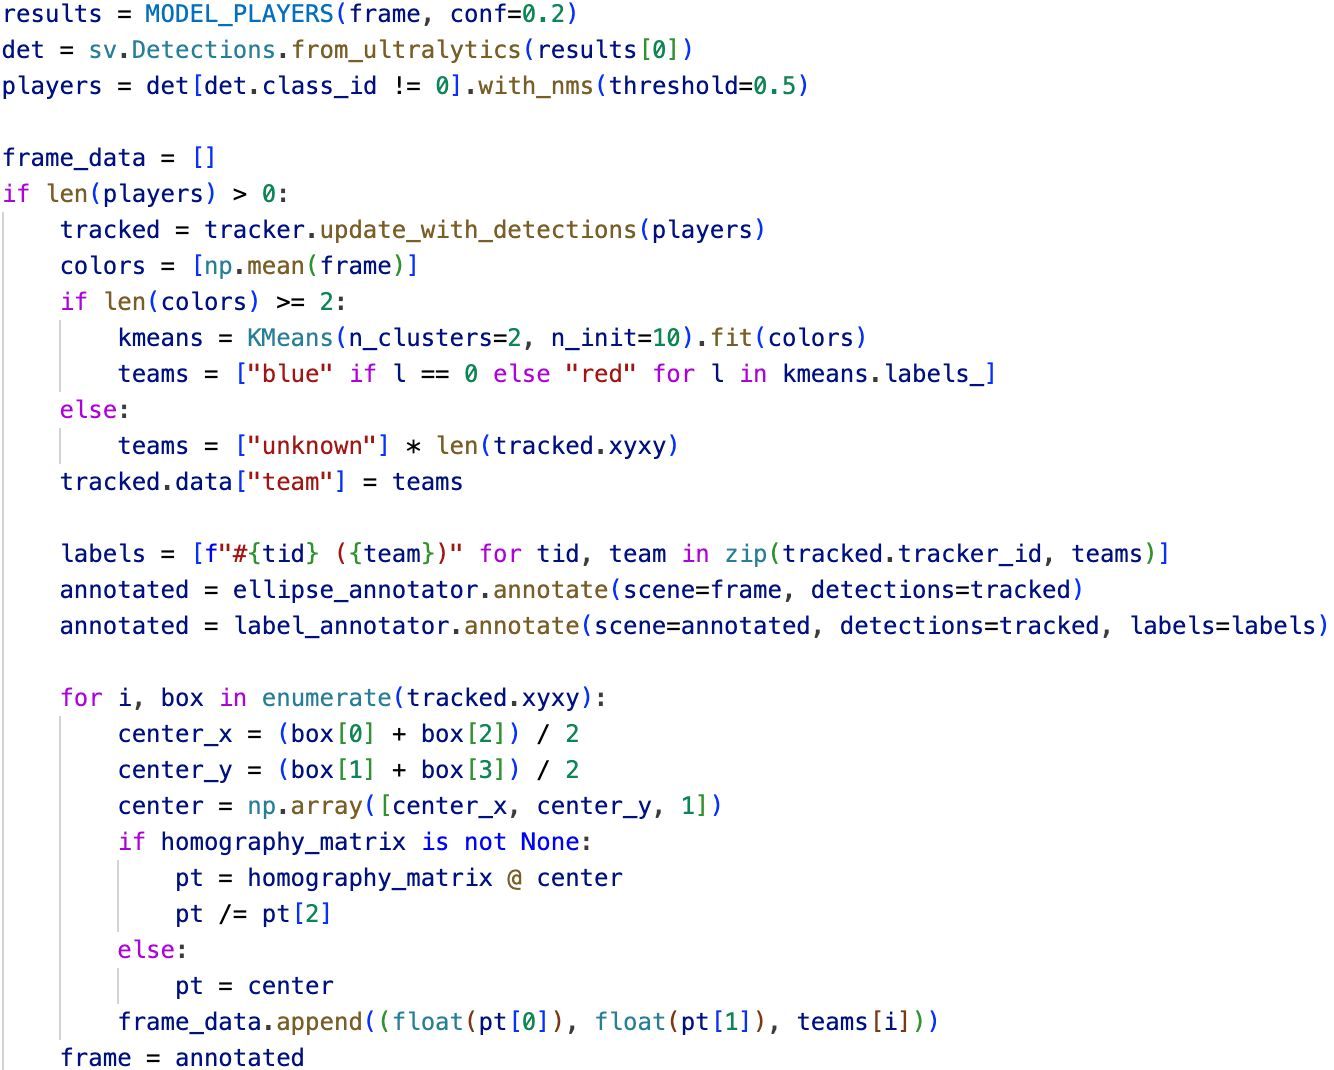
\includegraphics[width=0.9\textwidth]{figures/kmeans.jpg}
\caption{Python 3 code for frame analysis using YOLO and KMeans clustering}
\label{fig:enter-label}
\end{figure}


\begin{figure}[H]
\centering
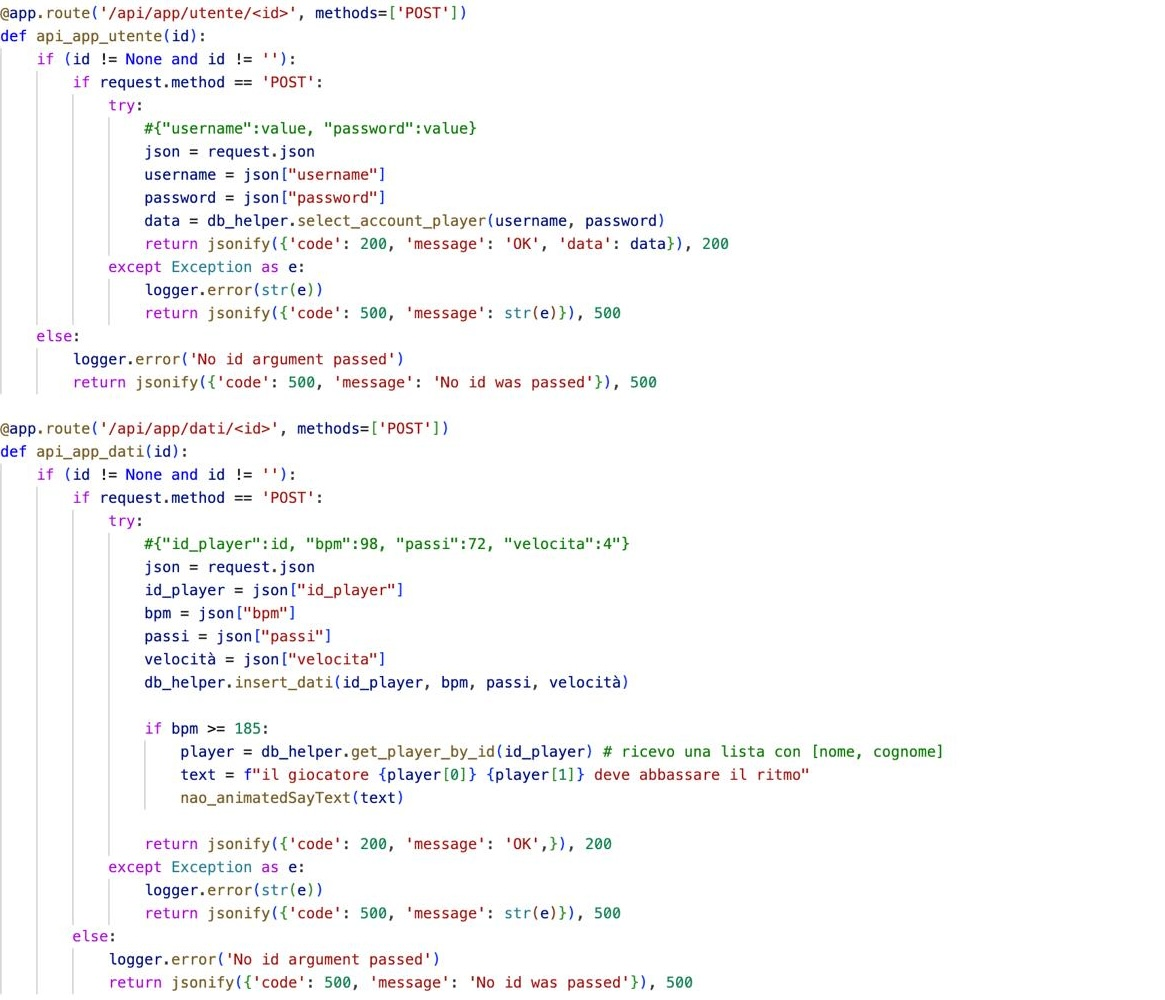
\includegraphics[width=0.9\textwidth]{figures/py3_2.jpeg}
\caption{Data storage in the database performed by the app}
\label{fig:py3_2}
\end{figure}

\FloatBarrier

\paragraph{Python 2 Pipeline}
Image acquisition from the NAO robot's webcam using ALVideoDevice, with parameterization (fps, resolution, brightness), and sending of the frame in JPEG format to the Python 3 server for later processing.

\begin{figure}[H]
\centering
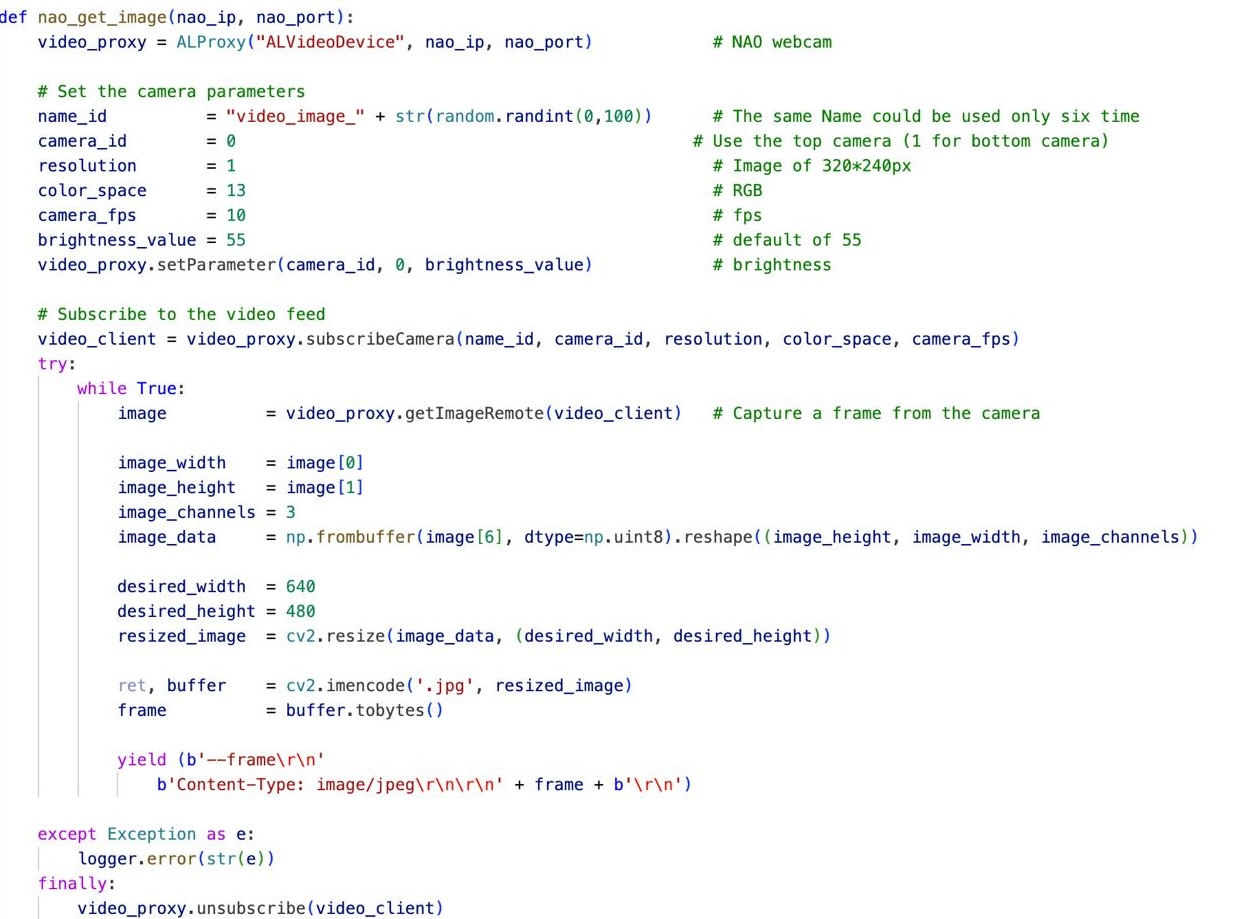
\includegraphics[width=\textwidth]{figures/py3_1.jpeg}
\caption{Python 2 code that receives input text and generates an MP3 audio file using the OpenAI library}
\label{fig:py2}
\end{figure}

\FloatBarrier


\paragraph{Video quality and analysis accuracy}
During testing phases, it emerged that using NAO's integrated camera presents limitations in terms of resolution and image quality. For this reason, recording matches with smartphones or professional video cameras was tested, obtaining better results thanks to higher clarity and video stability, which facilitate subsequent phases of computer vision analysis.
\FloatBarrier

\paragraph{Flask WebApp}
Management of authentication APIs and biometric data collection via HTTP POST requests from client or mobile application.

\subsection{General description of the application}
The application is designed for continuous and real-time monitoring of biometric parameters related to physical activity and the user's physiological conditions. The system enables the acquisition, transmission, and centralized management of data.

\subsection{Parameters detected by the app}
\begin{itemize}
    \item \text{Step count}: calculated using smartphone sensors, especially the accelerometer and gyroscope, which detect variations in the user's posture and movement. The processing occurs locally through a motor pattern analysis module.
    \item \text{Movement speed}: derived from GPS tracking through an algorithm that evaluates position variation over time, with possible time-based corrections to compensate for anomalies due to satellite signal or direction changes.
    \item \text{Heart rate (bpm)}: obtained from a wearable device that communicates wirelessly with the Google Fit platform. The application interfaces with this platform via REST APIs, periodically querying for updated data, then integrating it into the internal system.
\end{itemize}

\subsection{User interface}
Upon launch, the application presents the user with an intuitive graphical interface for authentication or registration, requesting mandatory identifying data, including first name, last name, unique player ID, and encrypted password. These data are processed in accordance with current personal data protection regulations with secure server-side storage.
\begin{figure}[H]
    \centering
    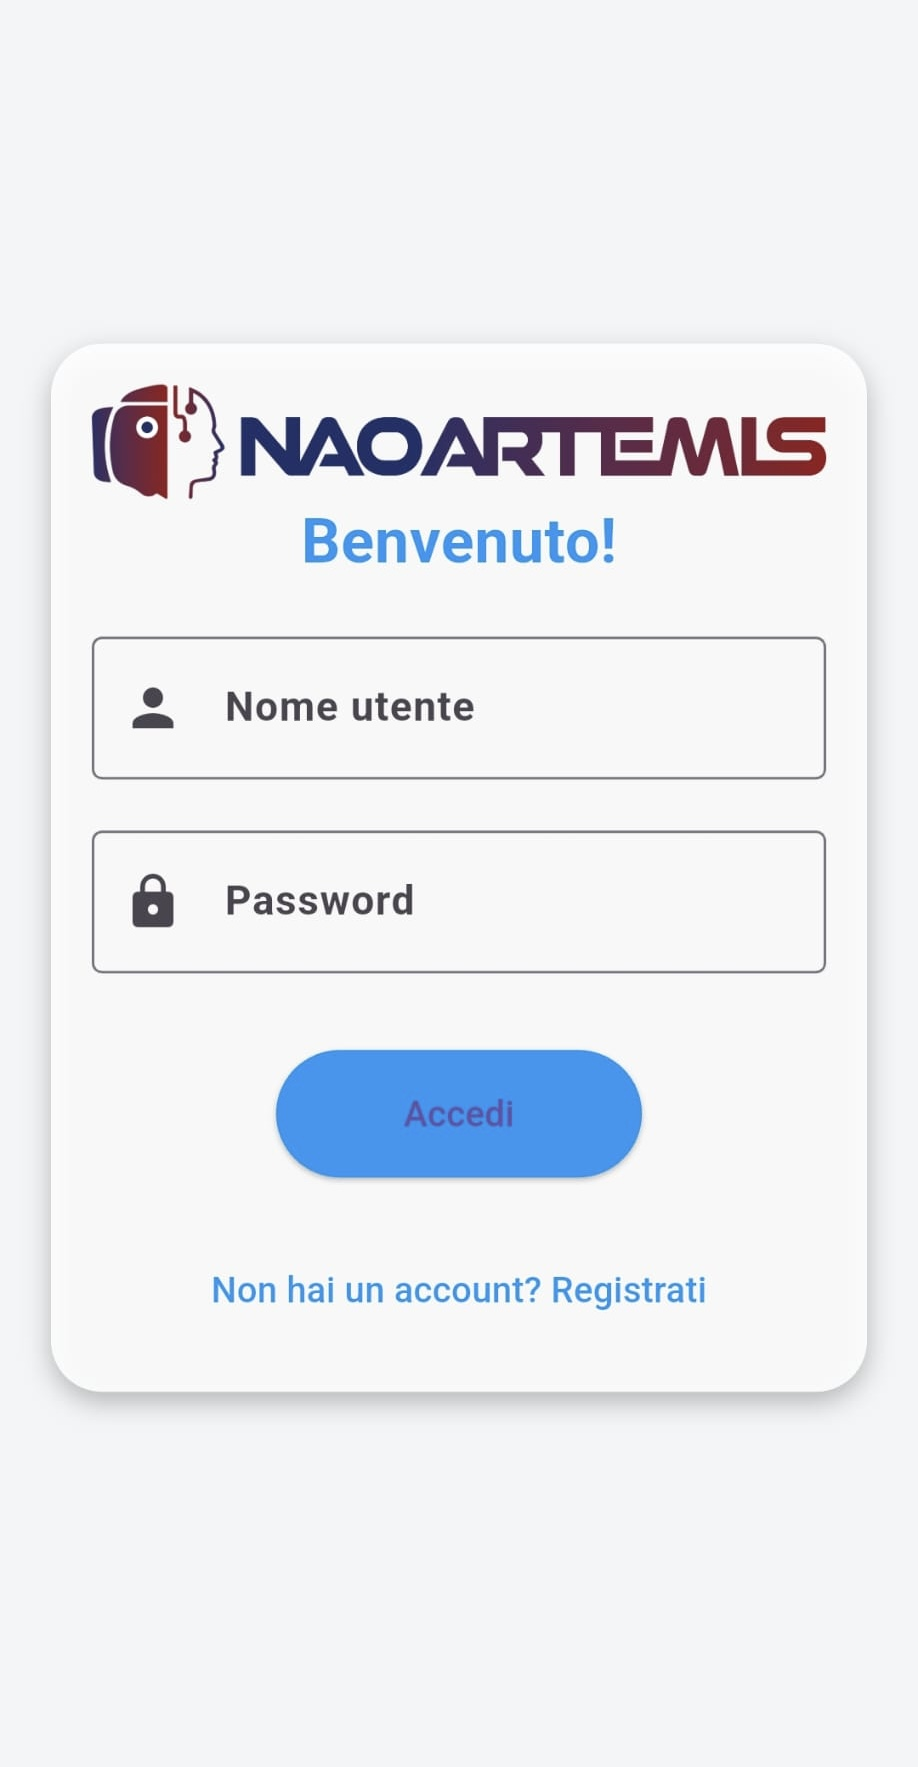
\includegraphics[width=0.5\textwidth]{figures/creaaccount_app.jpg}
    \caption{Login screen interface}
    \label{fig:registrazione}
\end{figure}

\subsection{Application infrastructure}
The application maintains a persistent connection (HTTP) with a remote server managing the application infrastructure and the following main functionalities:
\begin{itemize}
    \item \text{User authentication and authorization}: credential verification during login and controlled access to services.
    \item \text{Automatic synchronization of biometric data}: locally detected data are aggregated and periodically transmitted to the server based on a logic of time intervals or specific events (e.g., bpm threshold reached or significant position change).
    \item \text{Storage, validation, and analysis}: biometric data are stored in a centralized database, where they can be processed using algorithms to extract performance information, detect anomalies, or generate alerts.
    \item \text{Visualization}: the server infrastructure is set up to expose data to external dashboards, such as the webapp, capable of displaying graphs, maps, statistics, and individual histories useful for monitoring sports activity or users’ health status.
\end{itemize}
\bigskip

\section{Task 2 -- Inclusion, accessibility, and audience interaction}

\subsection{Positioning and access to the digital infrastructure}
During Task 2, the NAO robot is placed in the stands, in an elevated position, to obtain a panoramic view of the field and facilitate direct communication with the audience. In this configuration, NAO is connected to the Internet and integrated into a two-level distributed server architecture:
\begin{itemize}
    \item A Python 3 server, responsible for data processing, inference through artificial intelligence models, and database interfacing.
    \item A Python 2 server, which ensures compatibility with NAOqi proprietary APIs, required for low-level communication with the robot's hardware.
\end{itemize}
During this phase, NAO accesses the information processed in Task 1, querying the database via the Python 3 level.

\begin{figure}[h!]
    \centering
    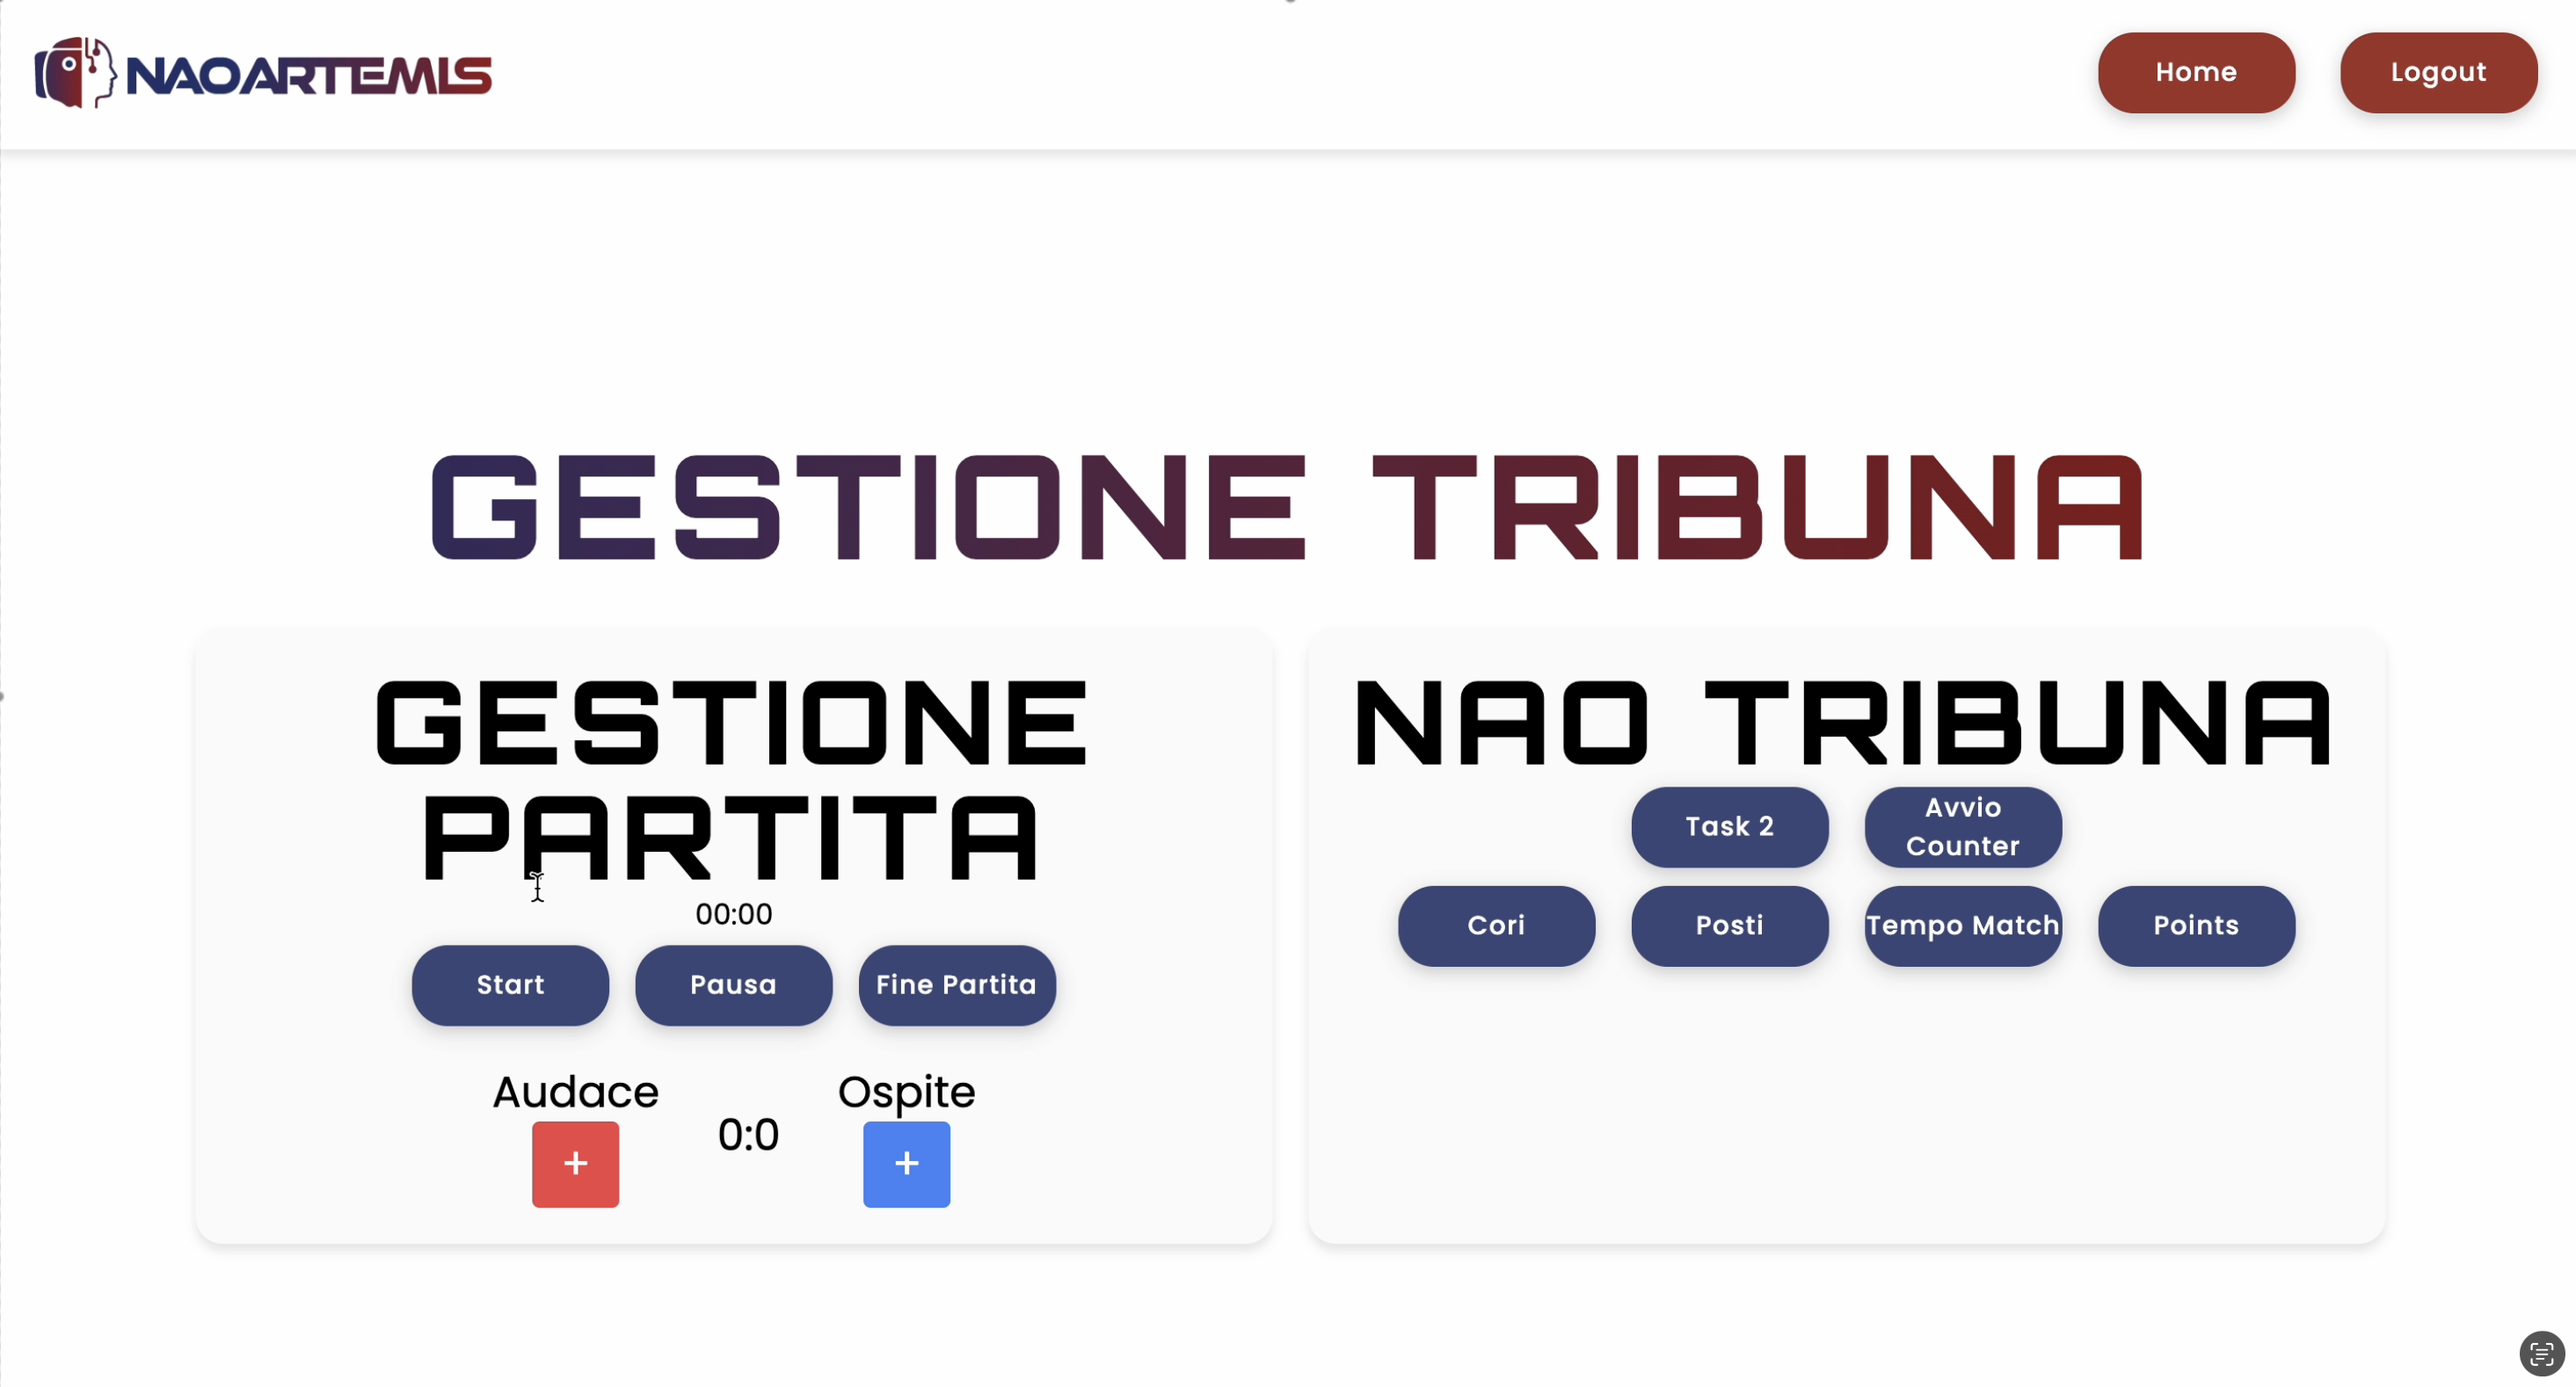
\includegraphics[width=0.95\textwidth]{figures/gestione_tribuna.png}
    \caption{Interface of the \textit{Stand Management} section, with controls dedicated to the match and functionalities accessible via NAO.}
    \label{fig:gestione_tribuna}
\end{figure}

\subsection{User interaction and enhanced accessibility}
The NAO robot acts as the main conversational interface for the user. To ensure a high level of communicative accessibility, particularly for users with disabilities, a paper-based system was designed using AAC (Augmentative and Alternative Communication). The AAC sheets contain:
\begin{itemize}
    \item Visually intuitive symbols and images.
    \item A visual ArUco marker, used to activate specific functions through visual recognition by NAO.
\end{itemize}
When the user shows a sheet containing an ArUco marker, the robot identifies it using its camera, decodes the associated ID, and activates the corresponding function on the Python 3 server. This server, if necessary, invokes procedures on the Python 2 server for direct interaction with the robot.

\subsection{Visual recognition through ArUco markers}
The choice of ArUco markers is justified by technical characteristics that make them optimal for complex environments:
\begin{itemize}
    \item High reliability in recognition.
    \item Faster detection compared to other visual codes.
    \item Ability to handle multiple markers simultaneously in the same frame.
    \item Robustness to rotations, distortions, and partial occlusions.
\end{itemize}
The project chose to use \textit{ArUco} markers instead of NAO’s native \textit{NaoMarks}. This decision was motivated by greater compatibility and stability offered by the open-source \textit{OpenCV} library, which includes a dedicated module for detecting and decoding ArUco markers.

Each ArUco marker is mapped to a specific function in the software system and represents a simple and effective way to command the robot without voice or touch interfaces.

\begin{figure}[h!]
    \centering
    
\includegraphics[width=0.25\textwidth]{figures/aruco.png}
    \caption{Example of ArUco marker used for recognition via computer vision.}
    \label{fig:aruco_marker}
\end{figure}

\subsection{Improving the voice system through advanced TTS modules}
To optimize communication between the robot and users, a \textit{Text-to-Speech} module based on OpenAI technology was integrated. This upgrade allowed for:
\begin{itemize}
    \item Improved quality and naturalness of the robot’s voice.
    \item Reduced frequency of pronunciation errors and increased clarity.
    \item More fluid and understandable voice communications, even in dynamic contexts.
\end{itemize}
Thanks to this integration, NAO is more effective and accessible in delivering messages, increasing inclusiveness and the impact of voice interactions.



\bigskip
\section{Beyond Code: NaoArtemis on Social Media}

\subsection{NaoArtemis: The Meaning Behind the Name — Robotics and the Future}
The name NaoArtemis is the fusion of the humanoid robot NAO — the technological protagonist of the project — and Artemis, the Greek goddess associated with strength, protection, and freedom. This choice is intentional: NAO represents the present of robotic innovation, while Artemis stands as a guiding ideal towards the future, symbolizing the balance between technology and humanity. The name thus reflects the project's mission: combining artificial intelligence, inclusion, and sports to support athletes and fans in an intelligent, ethical, and sustainable way.

\subsection{Visual Production Tools: From Graphic Design to Video Sets}
To develop the visual identity of the NaoArtemis project, the team adopted a professional approach, selecting suitable tools for digital and multimedia communication.

The official logos were designed using Adobe Illustrator, allowing for precise and consistent graphic elements.

For creating social media content — such as posts, stories, and carousels for Instagram, Facebook, and TikTok — Canva was used. This online collaborative tool proved especially effective for rapid and visually impactful graphics that aligned with the project’s branding. The use of custom templates, fonts, and palettes ensured uniformity and visual appeal across all channels.

Finally, promotional and demonstration videos were recorded on a professional photo set. This setting helped achieve high-quality content, enhancing the interaction with the NAO robots. The integration of technical tools and professional environments made NaoArtemis' communication not only effective but also aligned with modern multimedia production standards.

\begin{figure}[h]
  \centering
  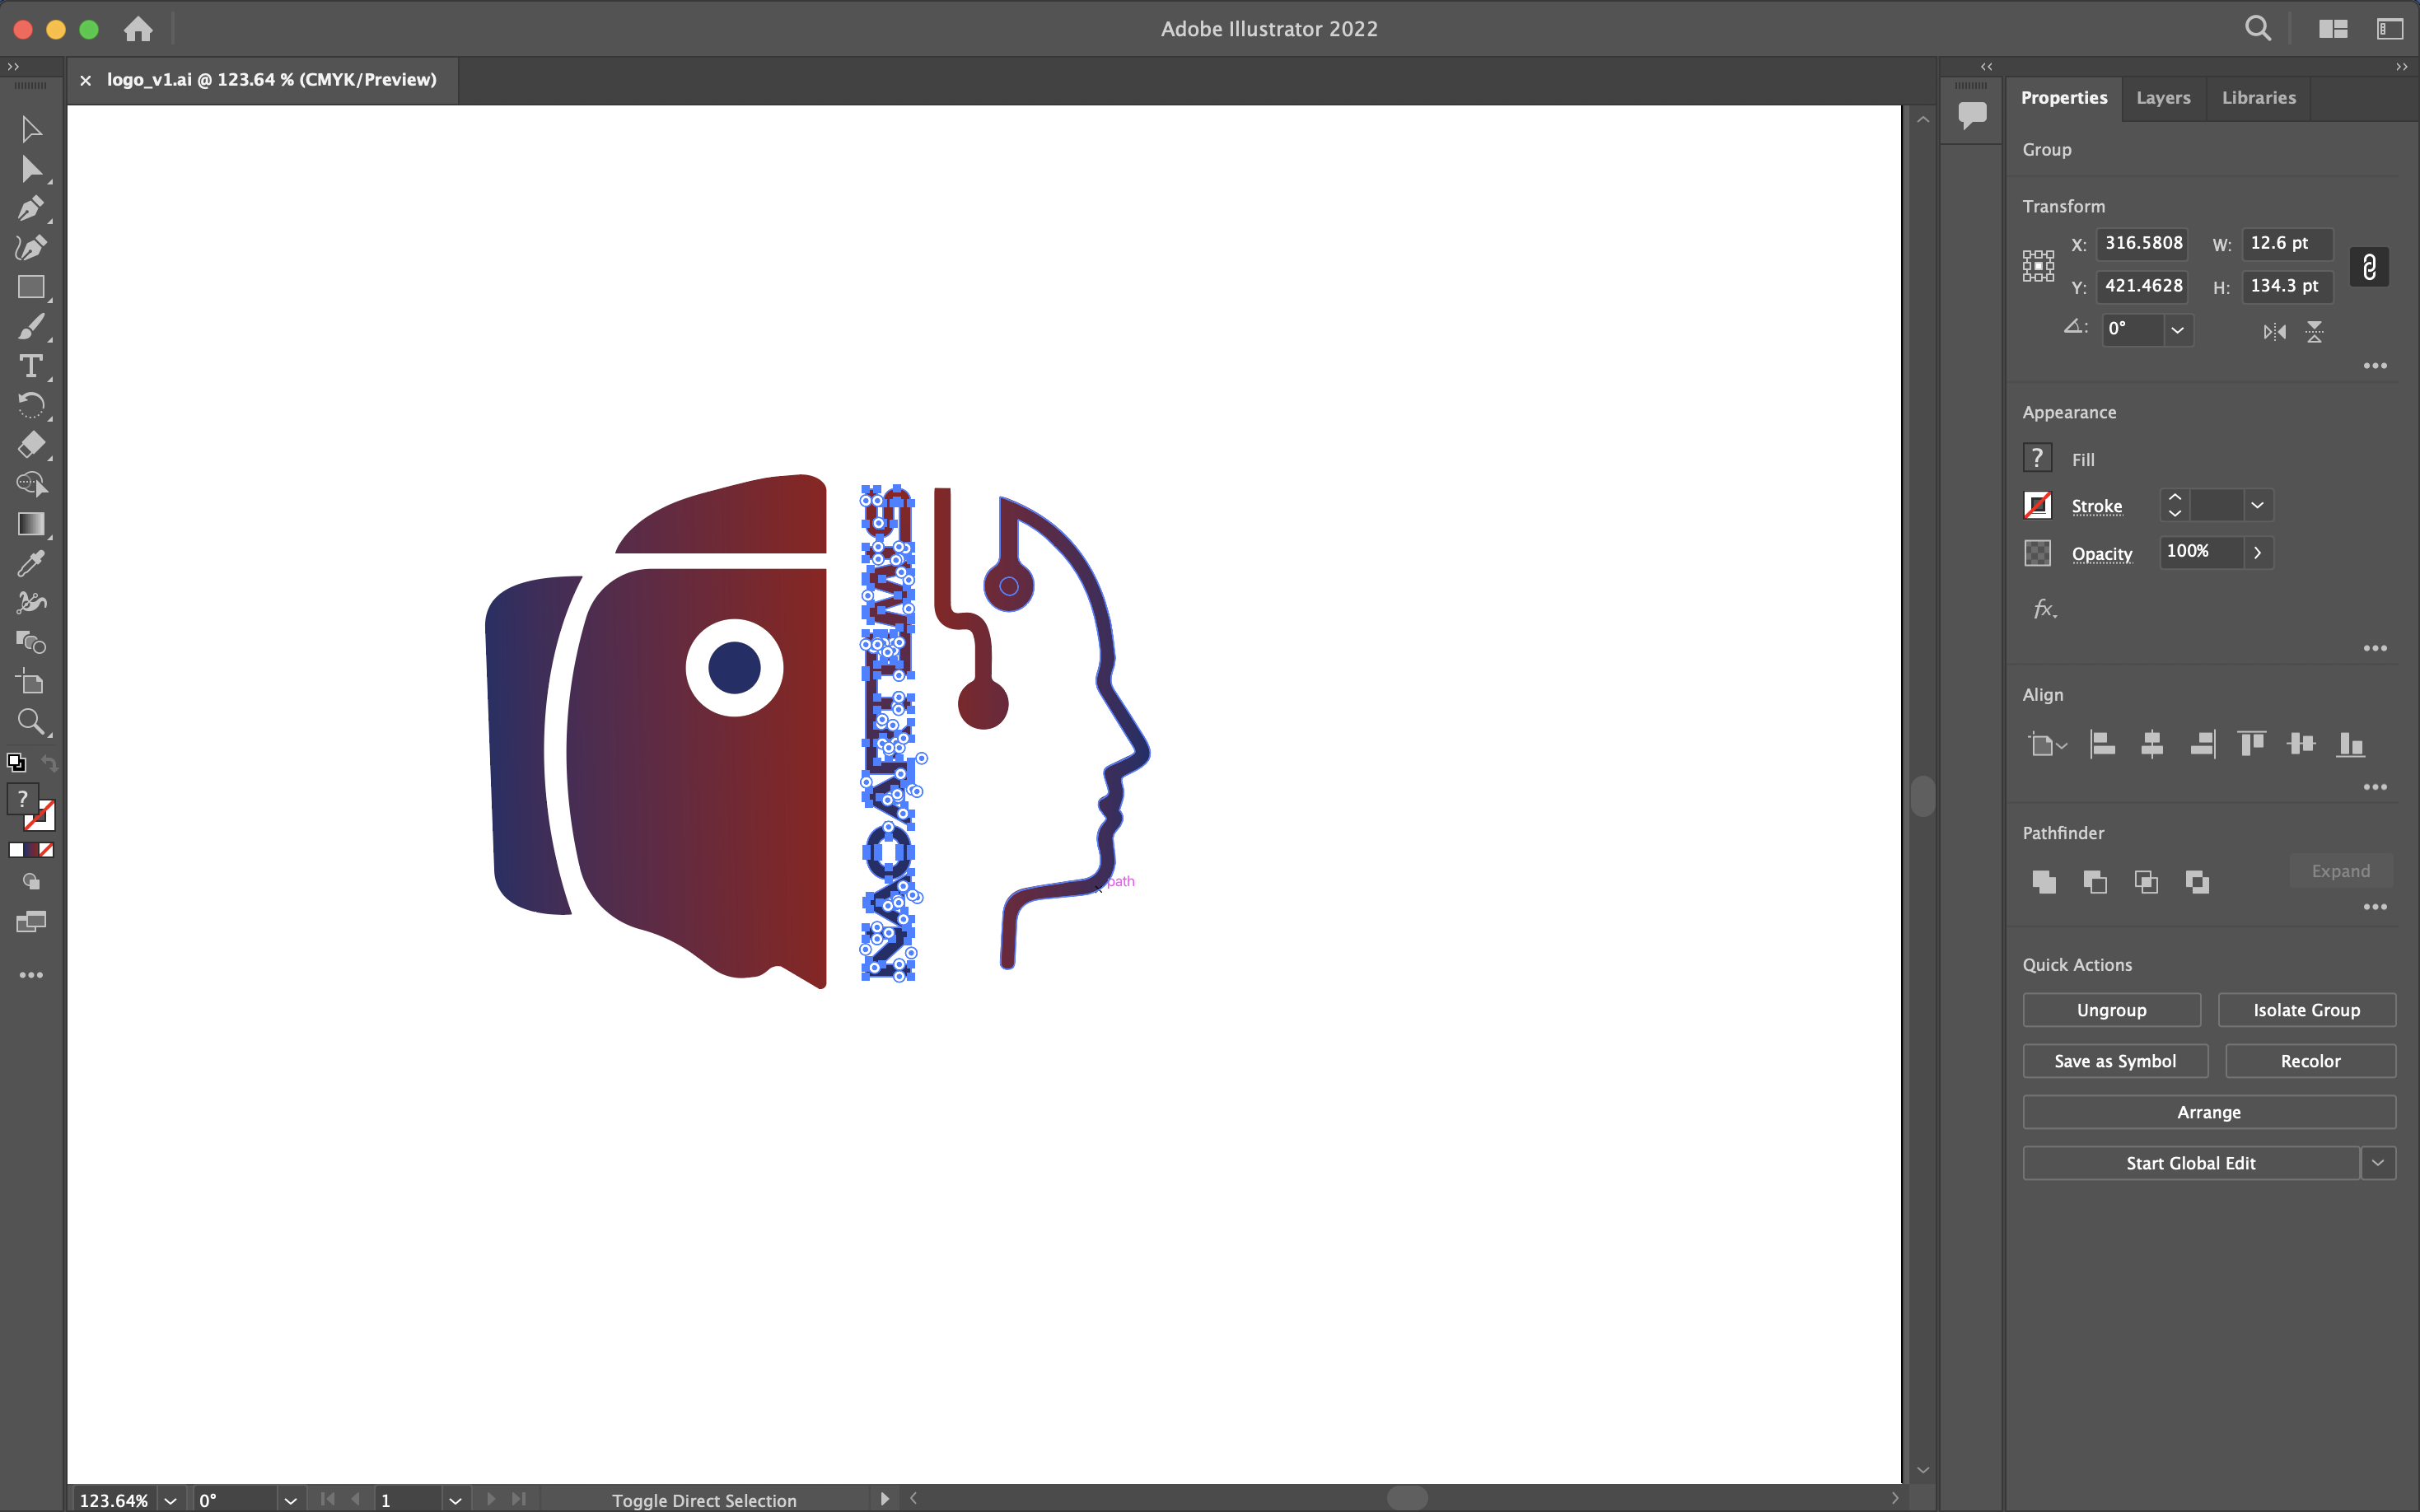
\includegraphics[width=\textwidth]{figures/illustrator.png}
  \caption{Illustrator}
  \label{fig:py3_01}
\end{figure}

\begin{figure}[H]
  \centering
  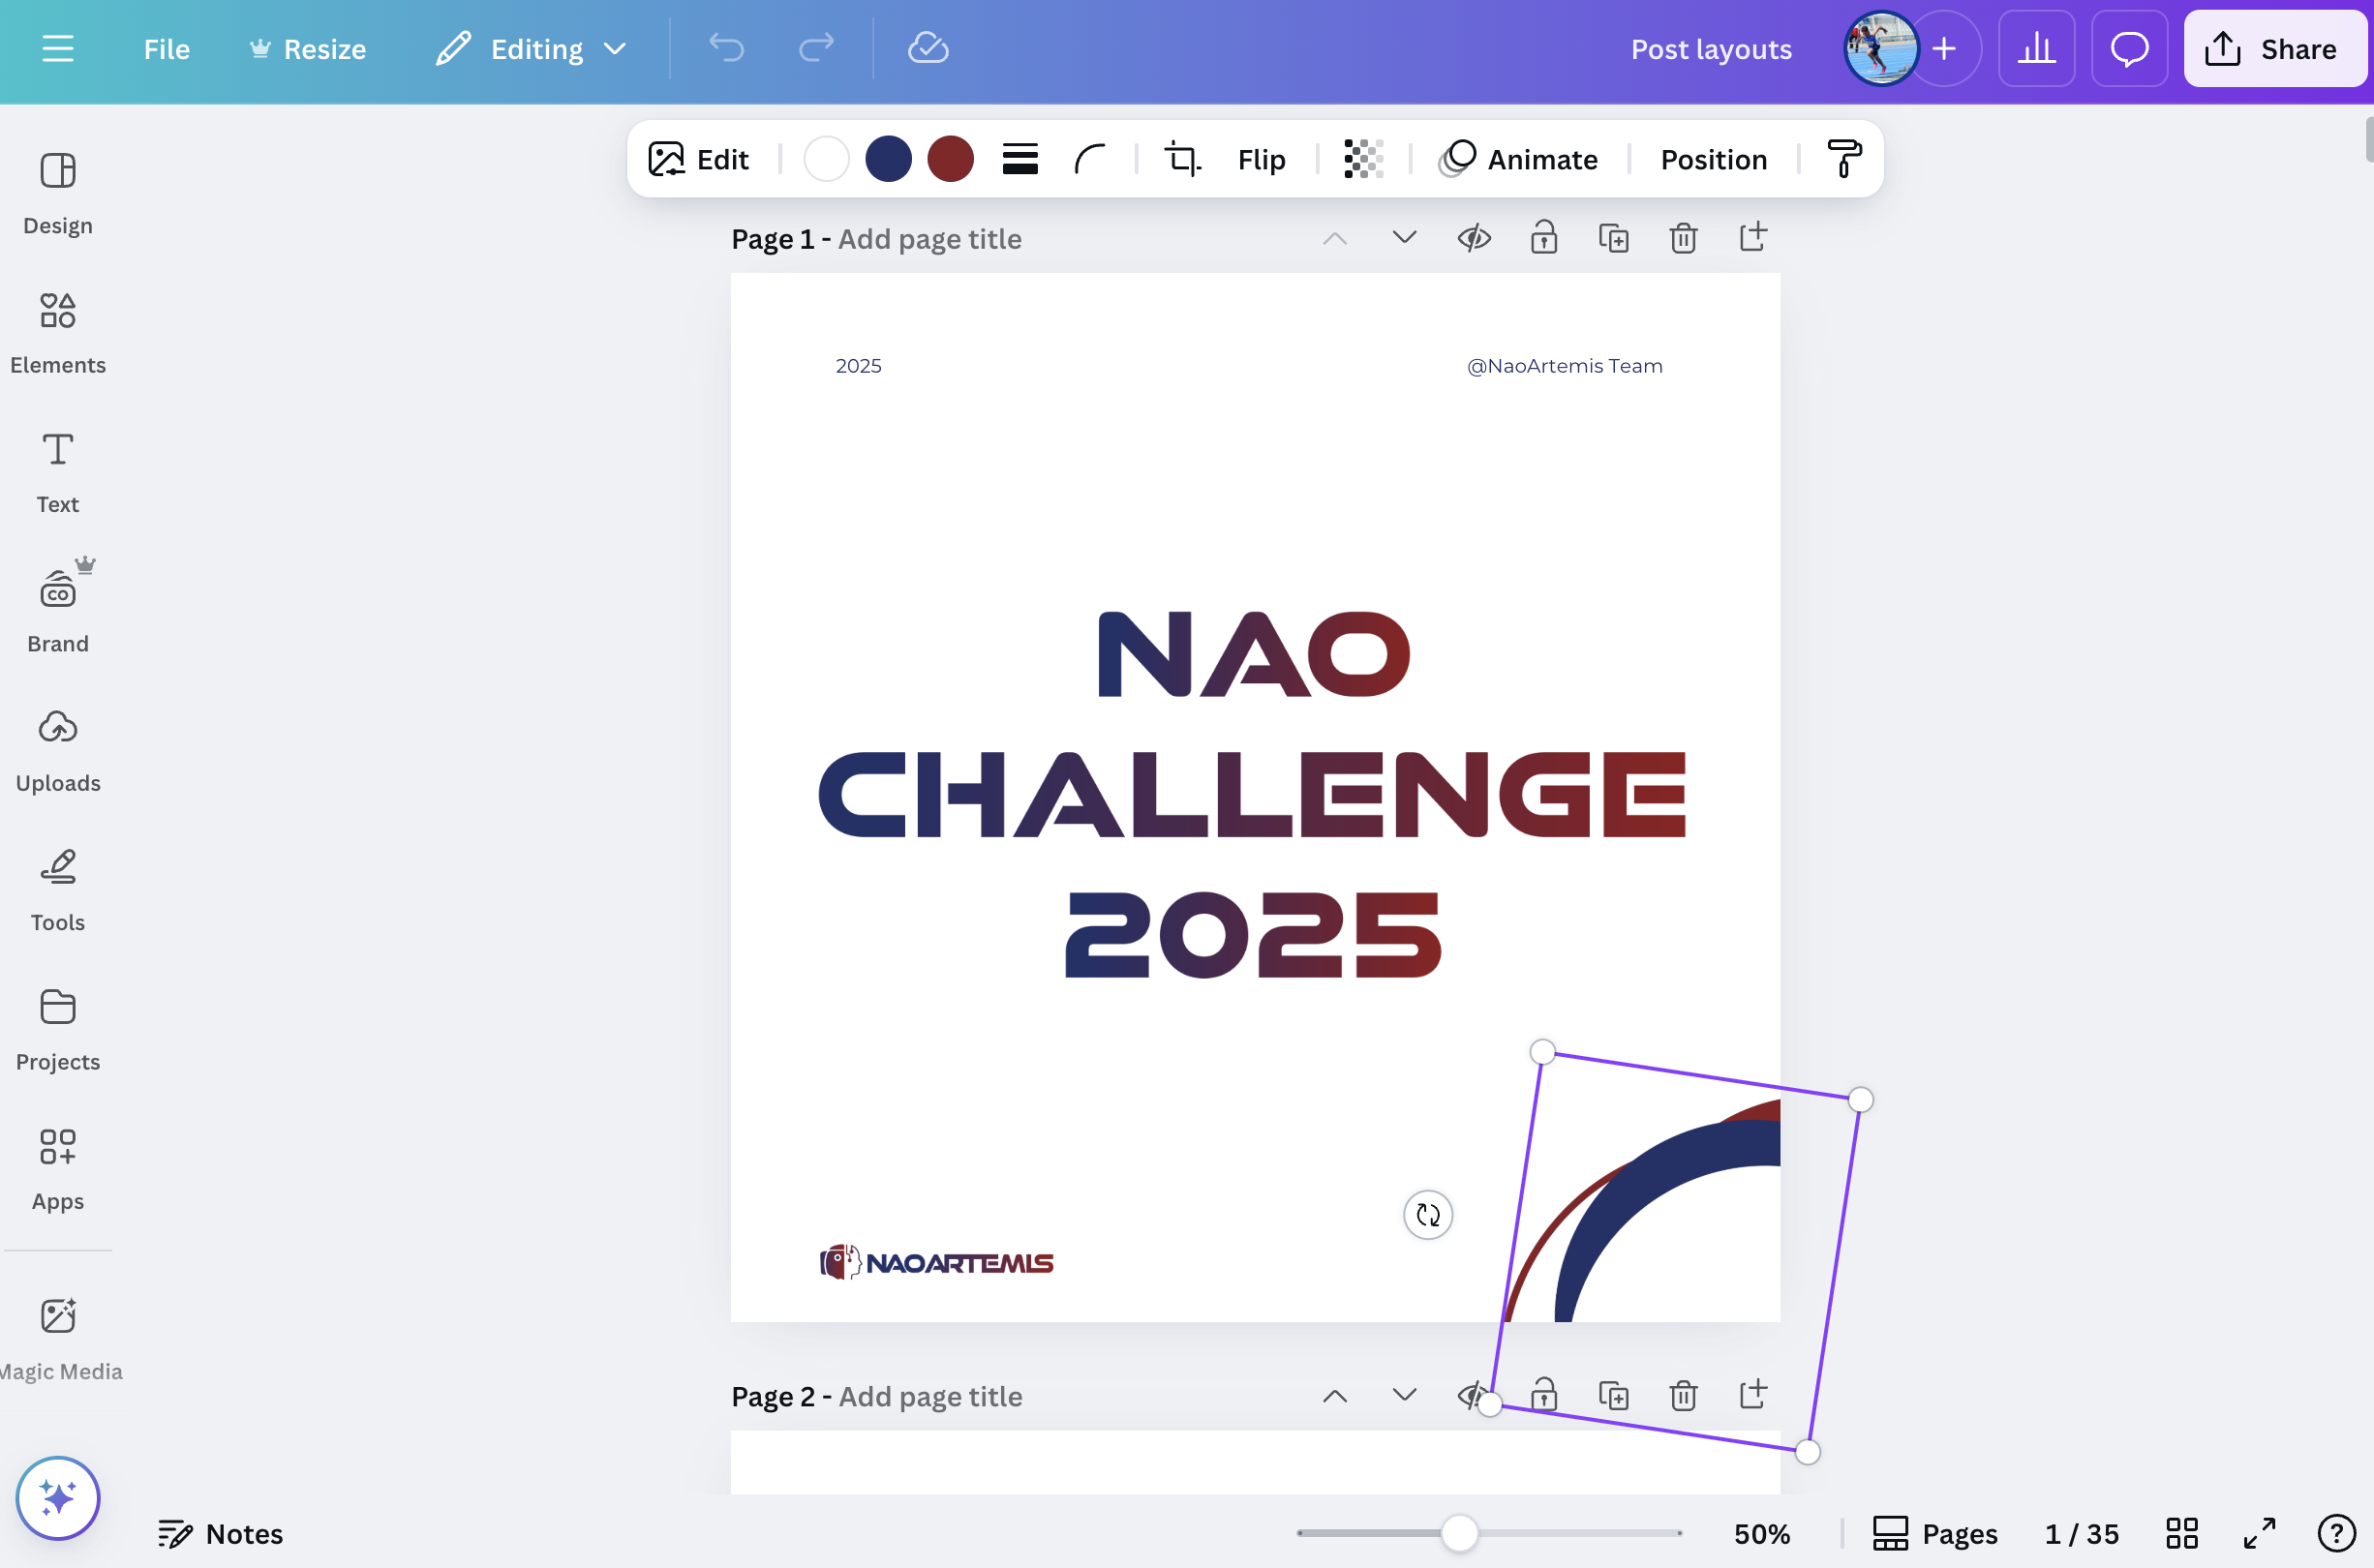
\includegraphics[width=\textwidth]{figures/canva.png}
  \caption{Canva}
  \label{fig:py3_01}
\end{figure}

\subsection{Visual Identity: Logo, Color Palette, and Typography}
The visual identity of NaoArtemis was designed to immediately convey the values of future, accessibility, and innovation.

The NaoArtemis logo is conceived to visually represent the essence of the project: the integration between technology and humanity.

The central element of the logo is the fusion between the stylized head of a NAO humanoid robot and the profile of a human face.

Connecting the two parts is a stylized neural network, a graphic element that represents artificial intelligence.

As a whole, the logo communicates future, inclusivity, and innovation — key values upon which the entire NaoArtemis project is founded.

To ensure communicative versatility and visual consistency across different contexts, the NaoArtemis team developed three distinct versions of its logo. Each version was designed to meet specific requirements of format, legibility, and visual impact, while maintaining a strong graphical unity.

\textbf{Logo 1 — Social Media Profile (Compact and Vertical Version)}\\
\begin{figure}[H]
    \centering
    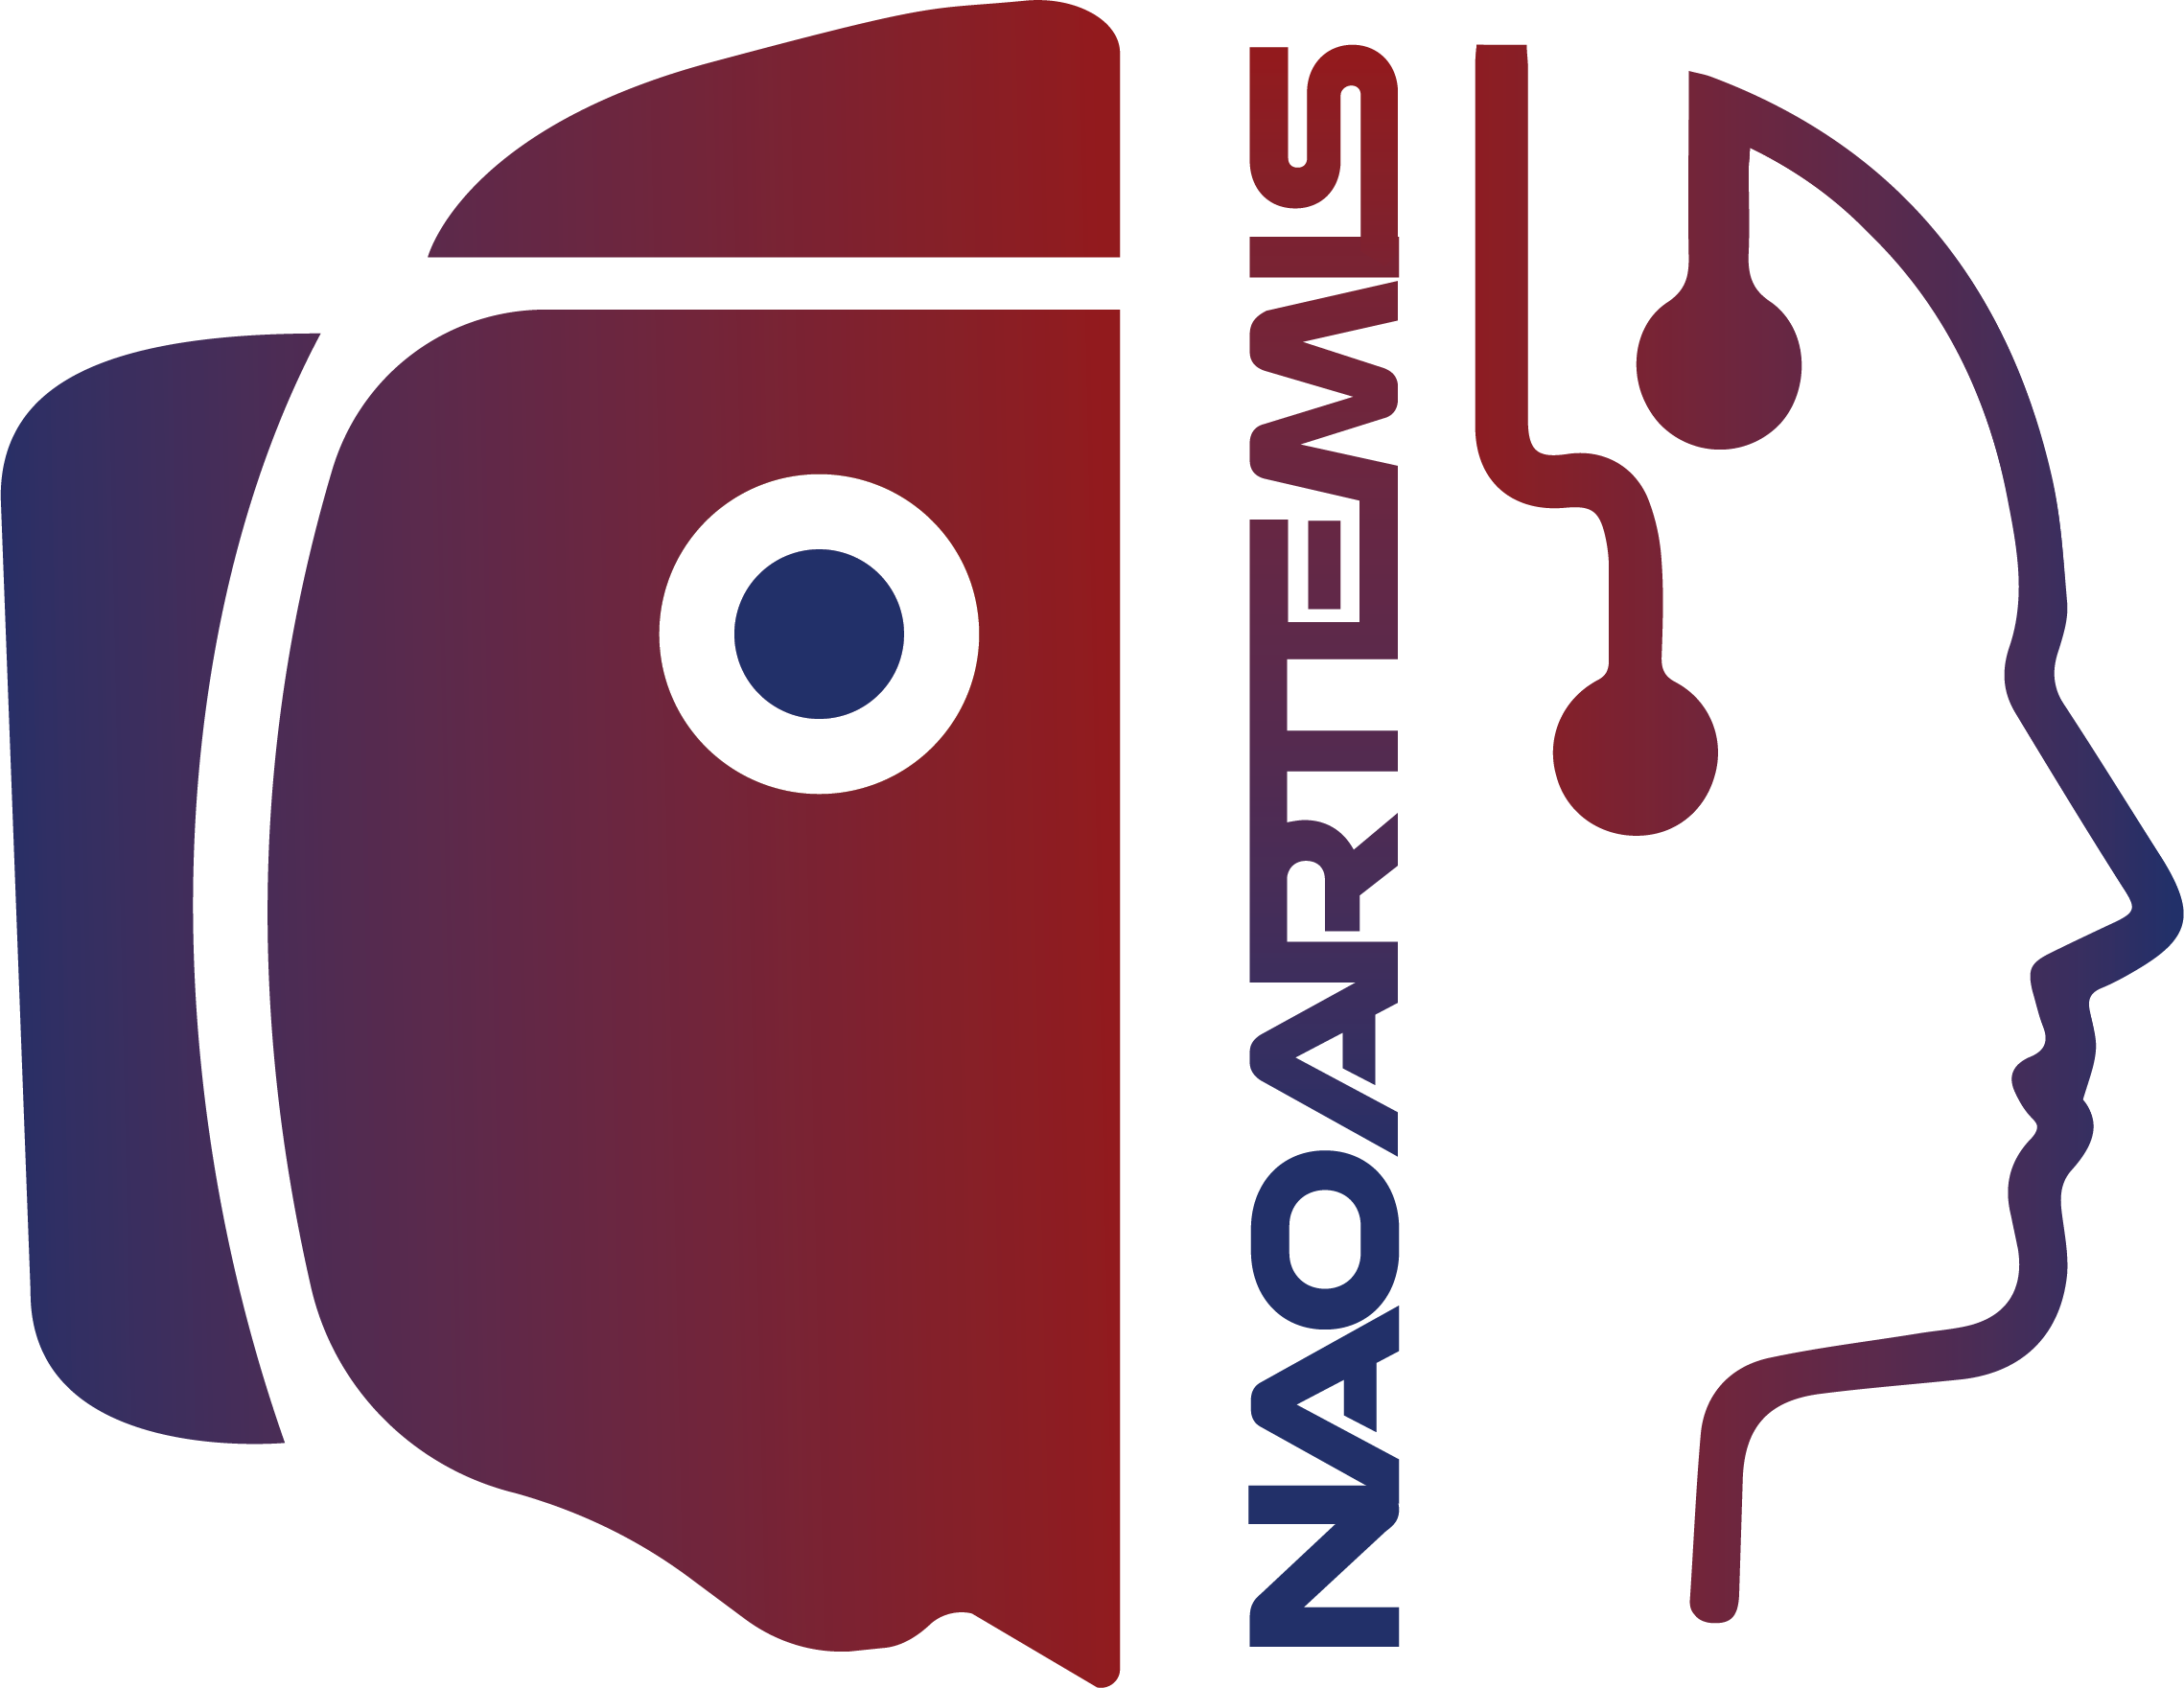
\includegraphics[width=0.2\textwidth]{figures/logo_v1.png}
    \caption{Logo version 1}
    \label{fig:logo_v1}
\end{figure}

This version is optimized for use as a profile image on social platforms (Instagram, Facebook, TikTok, YouTube). Thanks to its vertical format and compact composition, the logo retains clarity and recognizability even at small sizes. The project name is integrated vertically between the robotic silhouette and the human face.

\textbf{Logo 2 — Merchandising and Print (Centered Version)}\\
\begin{figure}[H]
    \centering
    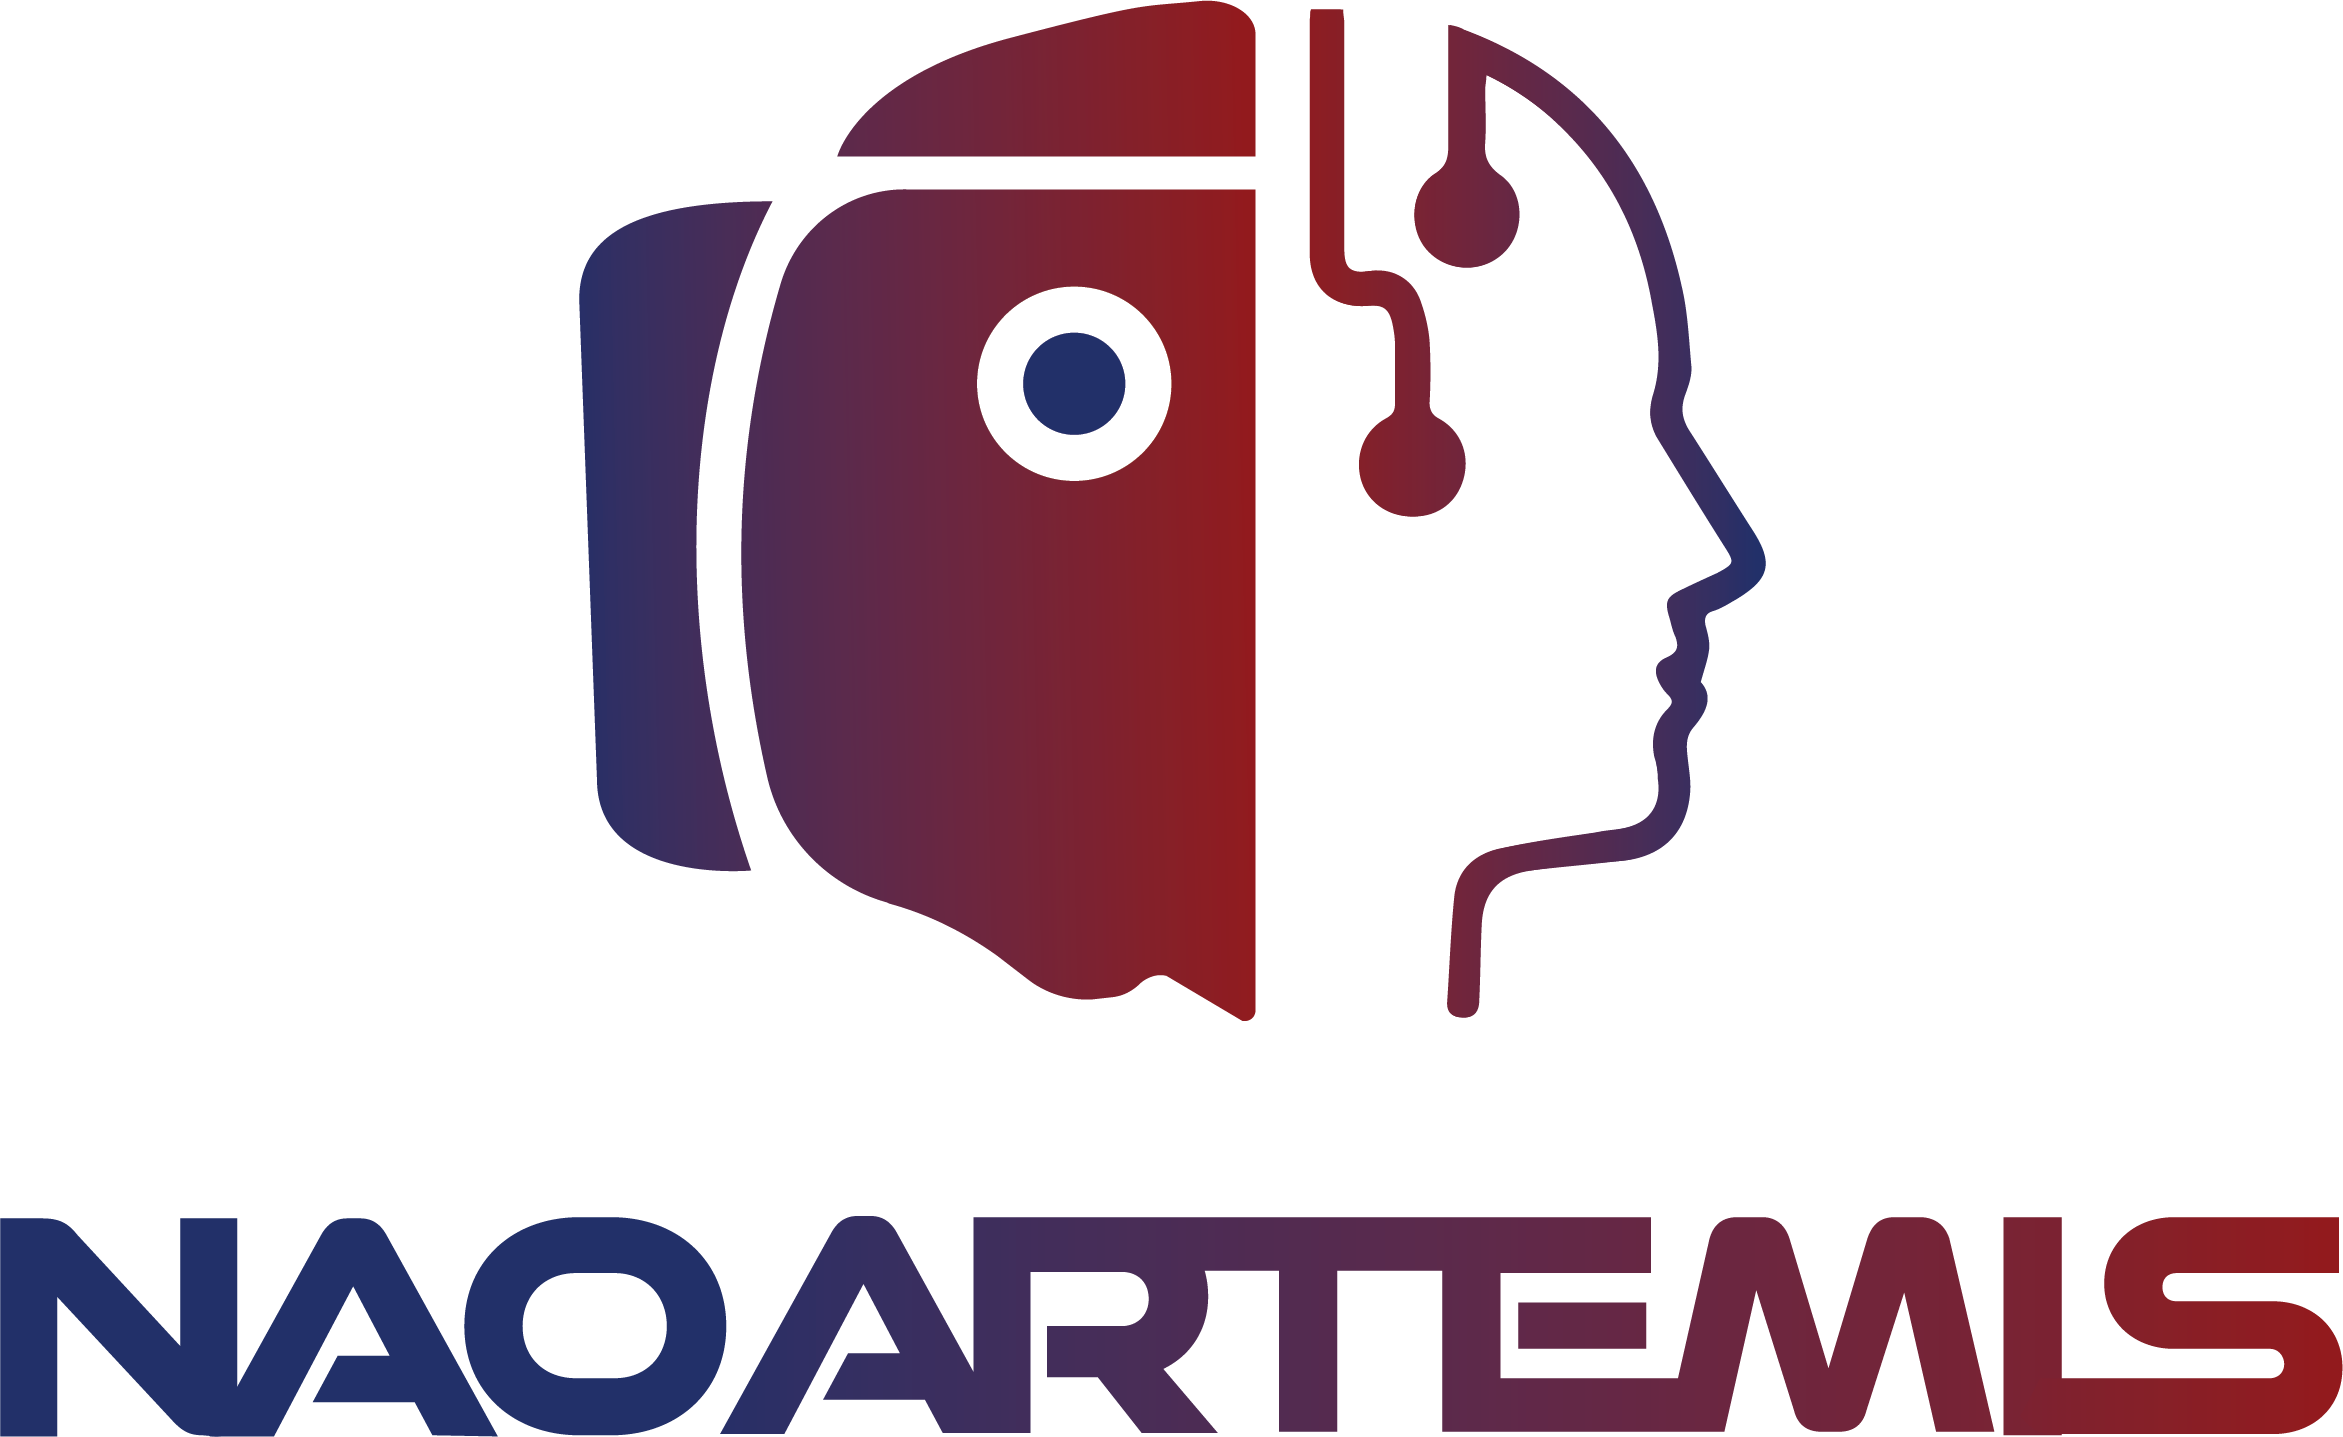
\includegraphics[width=0.3\textwidth]{figures/logo_v2.png}
    \caption{Logo version 2}
    \label{fig:logo_v2}
\end{figure}
Designed for physical materials such as t-shirts and business cards, this variant features a balanced composition between the graphic and the team name, with horizontal text for clear readability.

\textbf{Logo 3 — Official Communication (Extended Version)}\\
\begin{figure}[H]
    \centering
    
\includegraphics[width=0.5\textwidth]{figures/logo_v3.png}
    \caption{Logo version 3}
    \label{fig:logo_v3}
\end{figure}
Used in digital or editorial contexts where the team name should be prominently featured. The large "NAOARTEMIS" text alongside the composite icon is ideal for document headers and the website.

The color palette mainly uses shades of blue and red, sometimes with gradients as in the logo. The chosen fonts are Montserrat and Good Timing. Visual consistency across materials ensures strong brand recognition.

\subsection{Digital Presence: Strategic Social Media Management}
Online presence was developed across multiple platforms: Instagram, TikTok, Facebook, YouTube, and LinkedIn, each with content adapted to its audience and a shared editorial plan.

\textbf{Instagram}\\
Static posts, carousels, and bios to present the team, school, objectives, and partners; project descriptions in sequential posts; insights into sports, AI, inclusion, Audace, wellness, and performance; dynamic stories and themed reels.

\begin{center}
    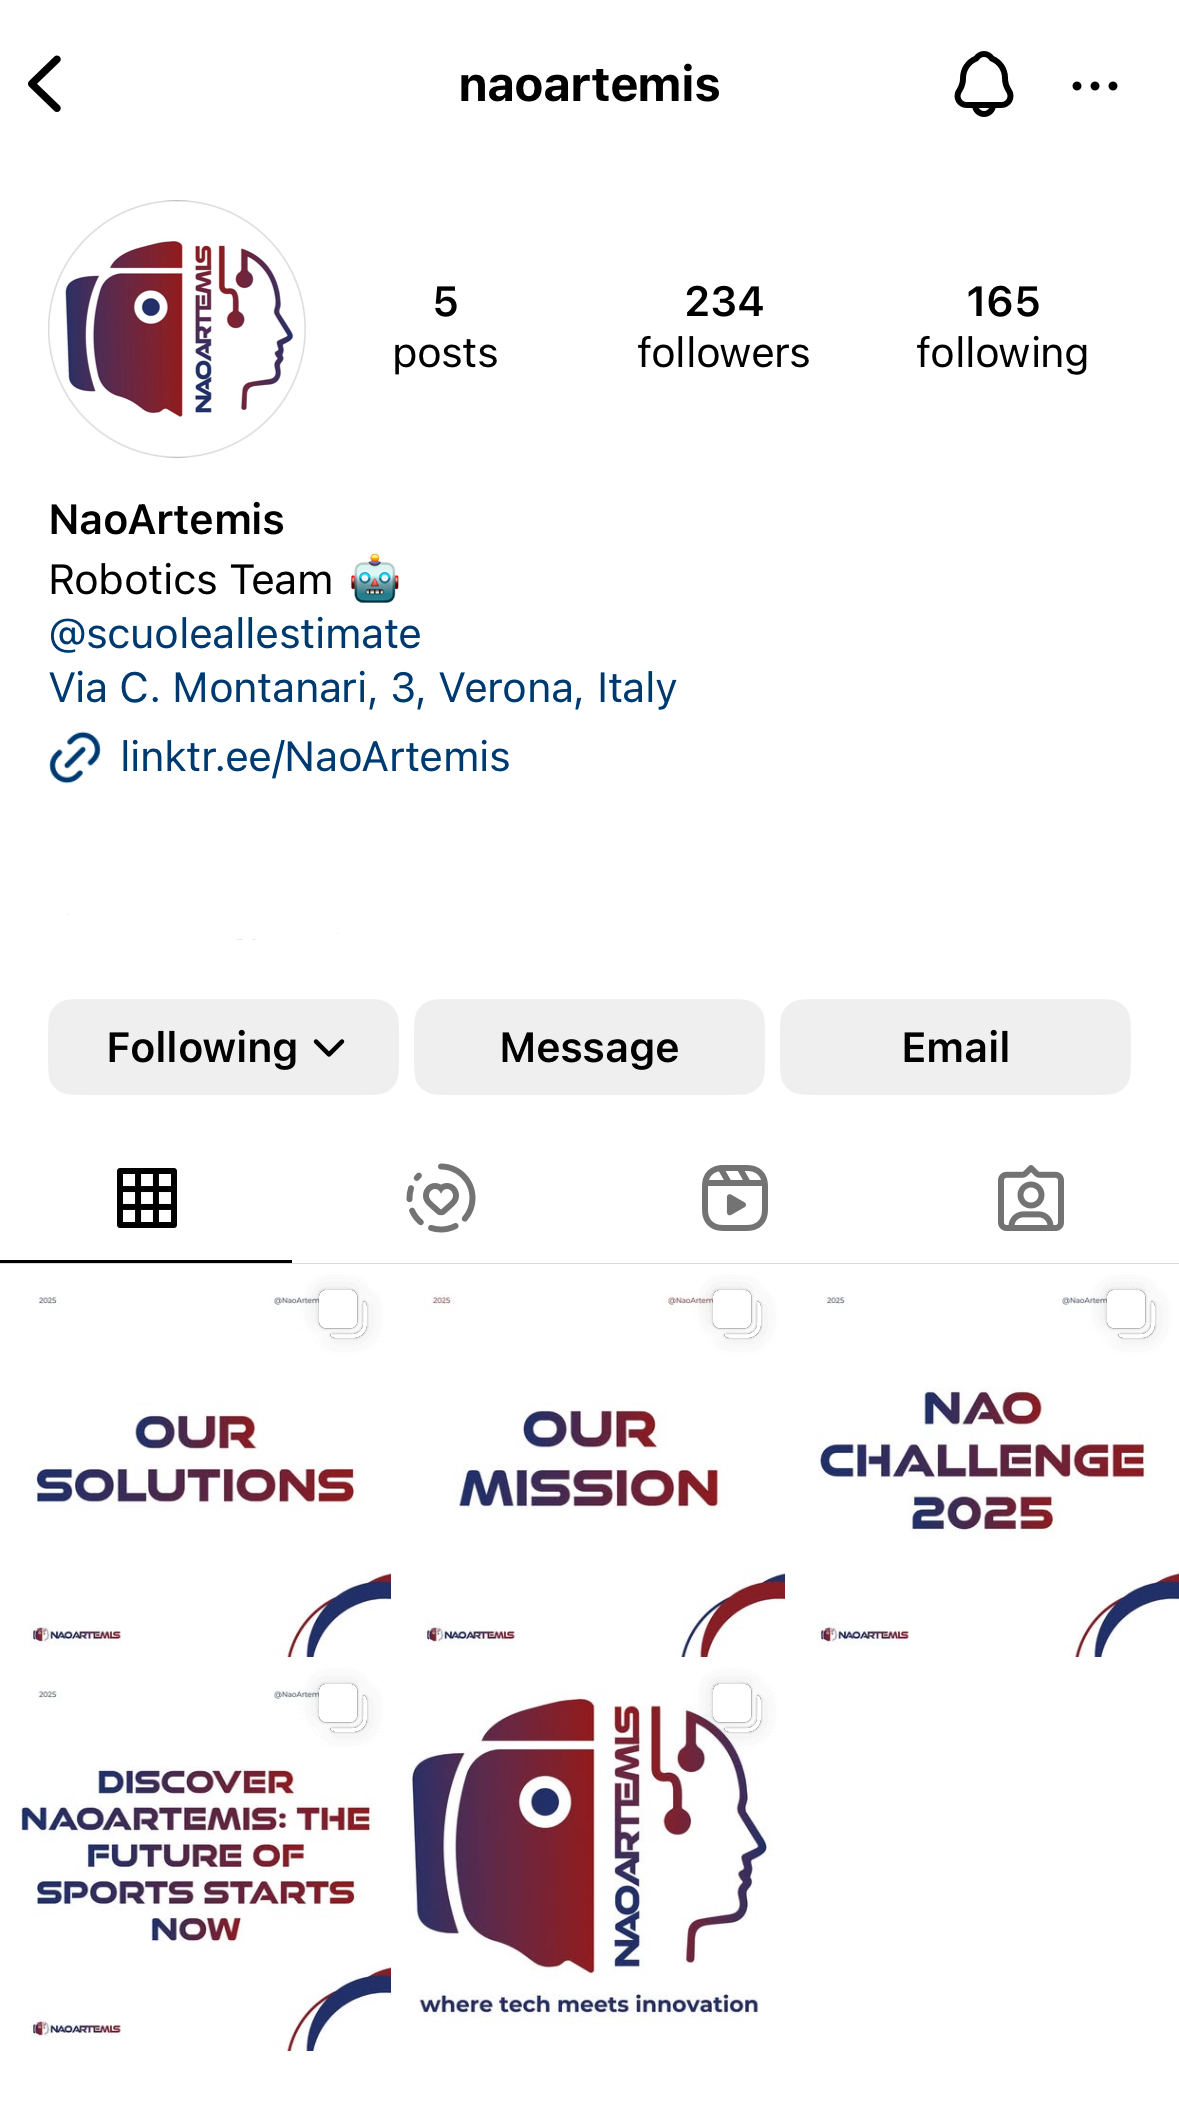
\includegraphics[width=0.4\textwidth]{figures/instagram.jpg}
\end{center}

\textbf{TikTok}\\
The same reels as Instagram, adapted to the platform’s format, focusing on speed, immediacy, and originality to attract a younger audience.

\textbf{Facebook}\\
Shared content with a more institutional tone, targeting parents, schools, and external partners.

\textbf{YouTube}\\
Collection of all published videos, plus a full video for official presentations and events.

\textbf{LinkedIn}\\
Used for professional and technical communication with teachers and companies.

Finally, Linktree was used — a useful tool in professional contexts — to organize and share a unified page containing links to all social channels.

\begin{center}
    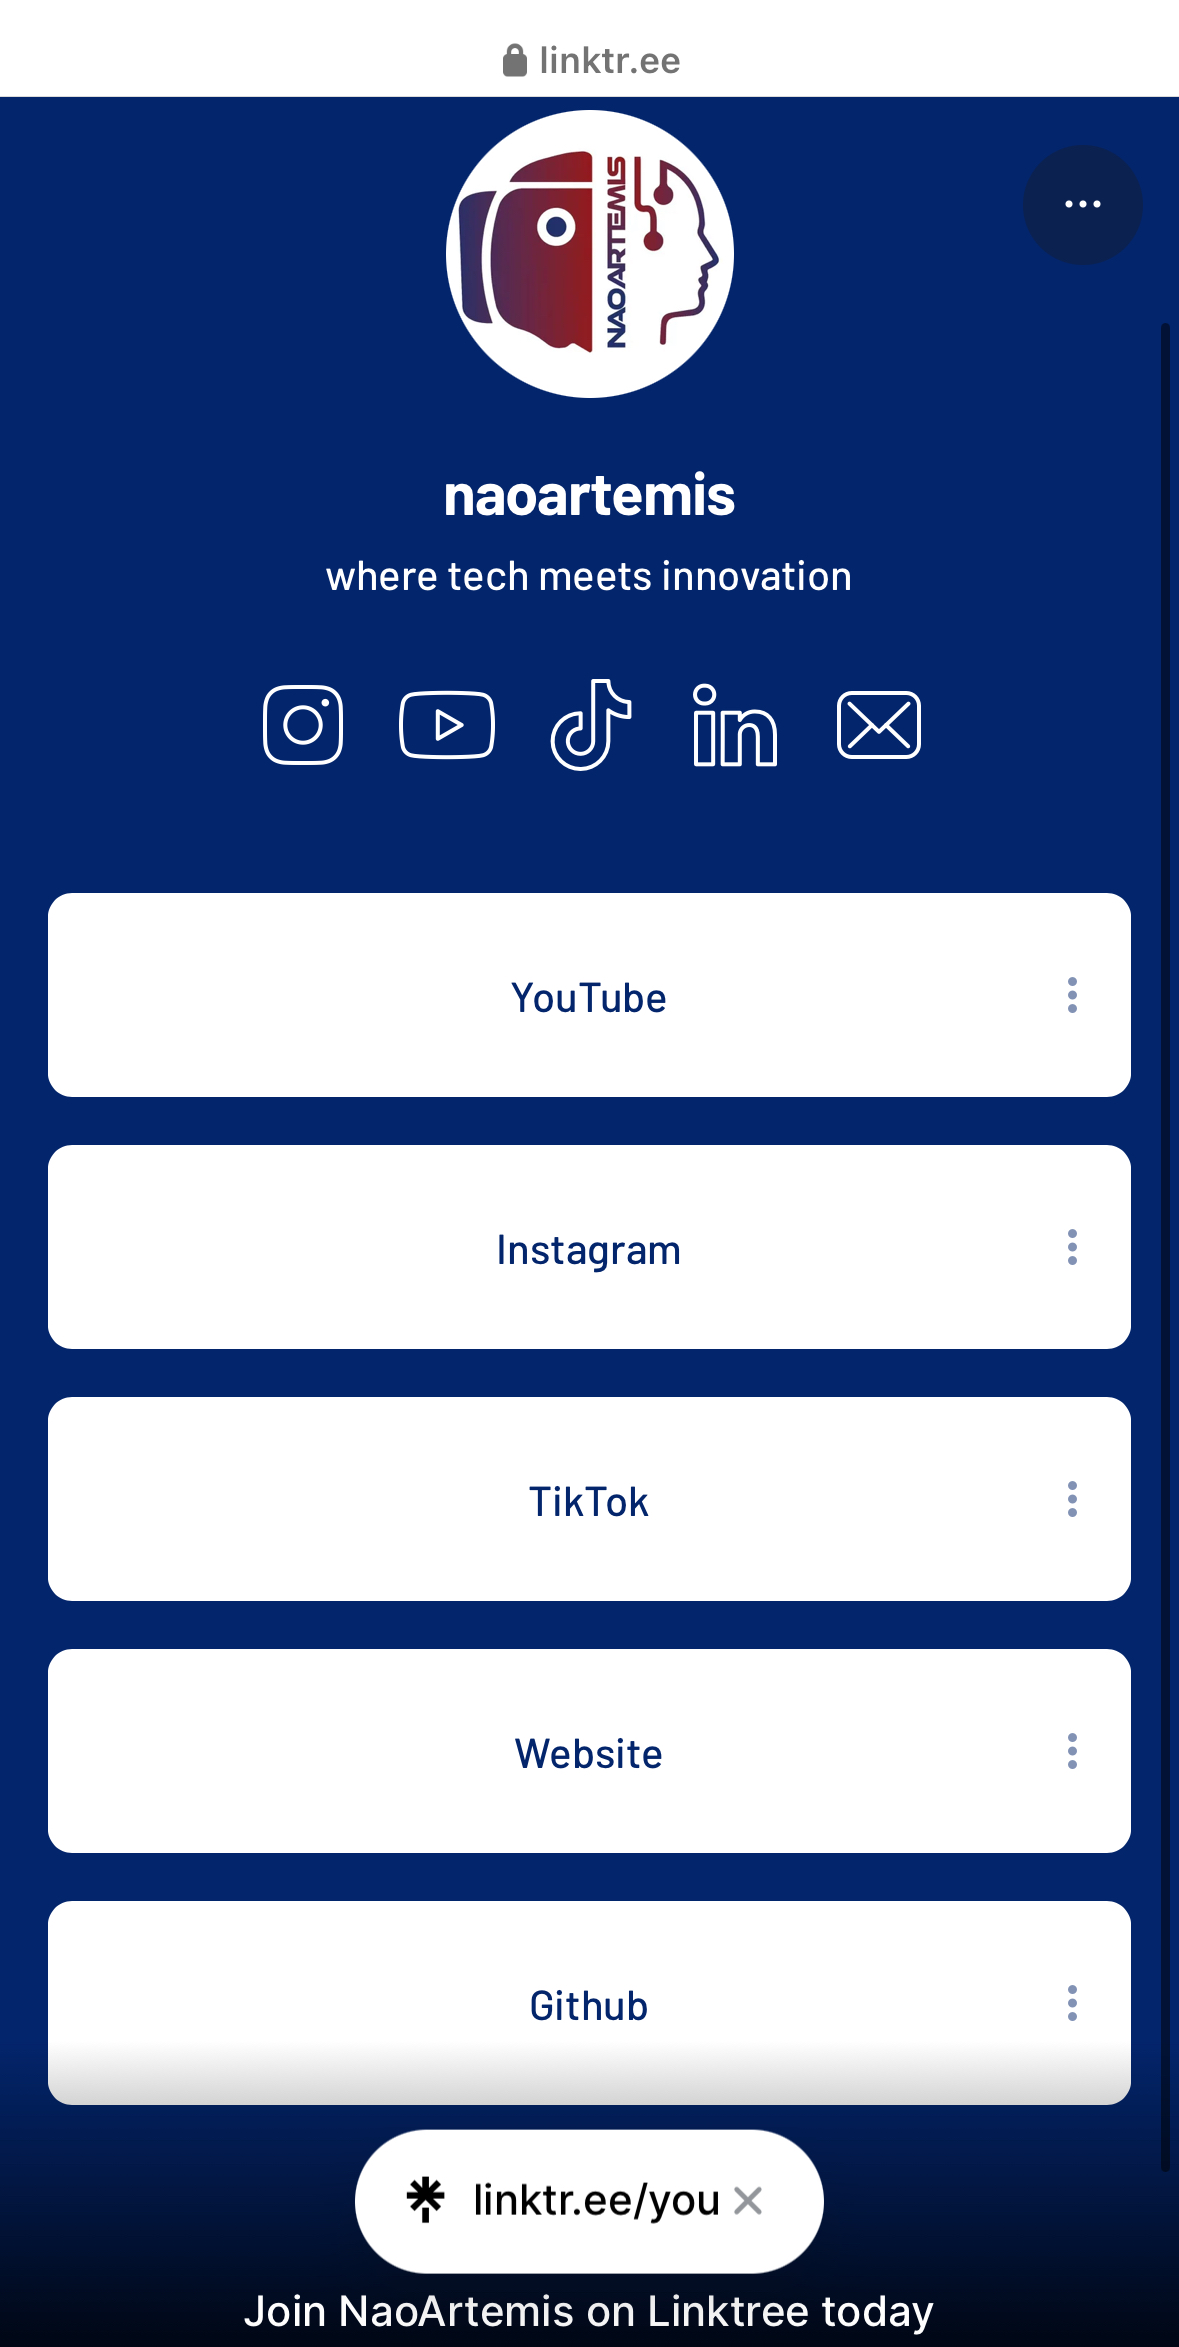
\includegraphics[width=0.4\textwidth]{figures/linktree.jpg}
\end{center}

\subsection{Web Platform: The Official NaoArtemis Website}

A dedicated website for the \text{NaoArtemis} project was created for the \text{NAO Challenge 2025}, documenting all core components of the initiative. It includes a \text{technical project description} structured around the two main tasks (sports training optimization and fan inclusion), team roles, and school affiliation. A section is also devoted to the \text{collaboration with the Audace sports club}.
\bigskip
\section{Team Members and Roles}

\subsection{Technology, Inclusion, and Education: The NaoArtemis Team at Stimate}
NaoArtemis was formed at Liceo “Alle Stimate” in Verona, a school with over two centuries of educational history, founded in 1816 by Saint Gaspare Bertoni. The institution stands out for its commitment to holistic education that combines academic excellence with the promotion of human, social, and spiritual values.

Within this context of innovation and openness, the school actively supports interdisciplinary projects like participation in the NAO Challenge. The NaoArtemis team, made up of students from the applied sciences program and led by Prof. Giovanni Bellorio, was born from this vision of combining technological passion, teamwork, and social commitment.

\subsection{Role Distribution}
\textbf{Giovanni Bellorio — Coach} \\Informatics teacher, team coordinator, and responsible for organizing and managing NAO Challenge activities.

\textbf{Mattia Begali — App Developer} \\In charge of app development for Task 1. Works on programming and integration of intelligent systems using Python.

\textbf{Laura Mascalzoni — Social Media Manager and Team Leader} \\Coordinates social platforms, manages multimedia content, and ensures consistency in communication.

\textbf{Giacomo Santi — Website Developer} \\Maintains the official website, ensuring accessibility, regular updates, and clear project presentation.

\textbf{Alessandro Albertini — Video Content Developer} \\Produces and edits video content. Manages the audiovisual pipeline and platform-specific adaptations.

\textbf{Alessandra Fiornini — Social Media Content Developer} \\Supports visual and textual communication on social media with precision and attention to detail.

\textbf{Haseeb Nabi — WebApp Developer} \\Advanced programmer for the NAO robot. Works on Task 1, computer vision, and the Web App.

\textbf{Marco Tomazzoli — NAO Programmer} \\Responsible for Task 2 features. Develops CAA-based interaction and ArUco symbol recognition.


\begin{figure}[b]
    \centering
    
\includegraphics[scale=0.08]{figures/logo_v3.png}
    \label{fig:logo_con_scritta1}
\end{figure}


%\vspace{70pt}
%\listoffigures
\end{document}